%%%%%%%%%%%%%%%%%%%%%%%%%%%%%%%%%%%%%%%%%%%%%%%%%%
%% Authors :    Giovanni Arcari                 %%
%%              Maria Bronzova                  %%
%%              Luca Sardi                      %%
%%              Spencer Sharp                   %%
%%                                              %%
%% Supervisor : Andreas Apostolatos             %%
%%											  	%%
%% e-mail : andreas.apostolatos@tum.de		   	%%
%%											  	%%
%% AFEM_group1_report.tex					  	%%
%%											  	%%
%%%%%%%%%%%%%%%%%%%%%%%%%%%%%%%%%%%%%%%%%%%%%%%%%%
\documentclass[a4paper,twoside,10pt]{article}
%%%%%%%%%%%%%%%%%%%%%%%%%%%%%%%%%%%%%%%%%%%%%%%%%%%%
%%											  	 %%
%% Author : Andreas Apostolatos               	 %%
%%											  	 %%
%% e-mail : andreas.apostolatos@tum.de		   	 %%
%%											  	 %%
%% packages.tex					  	   	 		 %%
%%											  	 %%
%%%%%%%%%%%%%%%%%%%%%%%%%%%%%%%%%%%%%%%%%%%%%%%%%%%%
\usepackage{amsmath}
\usepackage{amsthm}
\usepackage{amssymb}
\usepackage{makeidx}
%\usepackage{biblatex}
% Get support for the type font
%\usepackage{amsfonts}
% Get support for the subfigures
\usepackage{subfig}
% Get support for floating figures
\usepackage{float}
% Get support for mathematical symbols
\usepackage{mathrsfs}
% Get support for LaTeX graphics
\usepackage{graphicx}
% Disable ligatures
\usepackage{microtype}
\DisableLigatures[f]{encoding = *, family = * }
% Get support for multiple language packages
%\usepackage[greek,english]{babel}
%\usepackage[iso-8859-7]{inputenc}
\usepackage{mathptmx}
\usepackage{fancyhdr}
\usepackage{nopageno}
\usepackage{array}
\usepackage{multirow}
% Get support for the appendix
\usepackage{appendix}
% Get support for coloring parts of the text
\usepackage{xcolor}
% Get support for the bibliography 
%\usepackage[autostyle,german=guillemets]{csquotes}
\usepackage[style=numeric,sortcites=true,block=nbpar,backend=bibtex8]{biblatex}
% Adjust the geometry of the outcome pdf
\usepackage[a4paper,vmargin={27mm,23mm},hmargin={20mm,20mm}]{geometry}
\usepackage{physics}
\bibliography{literature}
\usepackage[utf8]{inputenc}
\begin{document}
    \pagenumbering{alph}
	%%%%%%%%%%%%%%%%%%%%%%%%%%%%%%%%%%%%%%%%%%%%%%%%%%%%%%%%
%%%%											  %%%%%%
%%%% 	Author: Andreas Apostolatos               %%%%%%
%%%%											  %%%%%%
%%%%	title_page.tex							  %%%%%%
%%%%											  %%%%%%
%%%%%%%%%%%%%%%%%%%%%%%%%%%%%%%%%%%%%%%%%%%%%%%%%%%%%%%%

% On the header of the title page
\thispagestyle{fancy}
\renewcommand{\headrulewidth}{0pt}
\lhead{}
\chead{}
\rhead{\footnotesize{Advanced FEM/FE-Technology\\
Dr-Ing. Roland W\"uchner}}
\pagenumbering{gobble}

% On the authors and the title of the project
%\long\def\symbolfootnote[#1]#2{\begingroup%
%\def\thefootnote{\fnsymbol{footnote}}\footnote[#1]{#2}\endgroup}
%\begin{center}\large{\textbf{A sample report in \LaTeX}}\\[10pt]\end{center}

\begin{center}\Large{\textbf{Advanced Finite Element Method - Assignment}}\\[20pt]\end{center}

\linespread{1.5}

\begin{center}\LARGE{\textbf{Sensitivity analysis for different objective functions in two-dimensional linear elasticity using standard finite elements}}\\[20pt]\end{center}

\vspace{3mm}

\begin{center}\large{\textbf{24/07/2019}}\\[10pt]\end{center}

\vspace{3mm}

%\begin{center} \textbf{Authors}$^{\mathbf{1}}$\\[5pt]\end{center}
\begin{center} \large{\textbf{Authors}}\\[10pt]\end{center}

\begin{center}\large{Arcari Giovanni}\\[10pt]\end{center}
\begin{center}\large{Bronzova Maria}\\[10pt]\end{center}
\begin{center}\large{Sardi Luca}\\[10pt]\end{center}
\begin{center}\large{Sharp Spencer}\\[10pt]\end{center}

\vspace{5mm}
\linespread{1}

\begin{center}\large{M.Sc. students in Computational Mechanics\\
Technical University of Munich}\\[10pt]\end{center}



\newpage
	
	%%%%%%%%%%%%%%%%%%%%%%%%%%%%%%%%%%%%%%%%%%%%%%%%%%%%
%%											  	 %%
%% Author : Andreas Apostolatos               	 %%
%%											  	 %%
%% e-mail : andreas.apostolatos@tum.de		   	 %%
%%											  	 %%
%% 00_Abstract.tex					  	   	     %%
%%											  	 %%
%%%%%%%%%%%%%%%%%%%%%%%%%%%%%%%%%%%%%%%%%%%%%%%%%%%%
\section*{\normalsize{ABSTRACT}}

\pagenumbering{arabic}

\textit{The goal of the assignment is to develop and run sensitivity analyses for different objective functions for a 2-dimensional linear elasticity problem with standard finite elements. Finite element code was provided as a basis on which to develop the sensitivity analysis. Three different types of sensitivity analyses were implemented - global, semi-analytical, and analytical - for three different objective functions - strain energy, displacement, and Von Mises stress.  As an input for the calculations, a set of nodal displacement is taken; the results illustrate how they affect the analyzed objective functions. To perform each calculation, finite differencing methods are used. For all of the analyses, a single reference case, in terms of geometry, loading, boundary conditions, and material properties, is considered. A convergence study was performed in order to ensure a proper perturbation value was chosen for the nodal displacements. The code was validated by a comparison of results from the various types of sensitivity analyses that were implemented. Finally, the sensitivity analysis was utilized to perform a relatively simple optimization of the given geometry.}\\%IT SHOULD BE AROUND 200 WORDS -> CHECK! ->THIS SHOULD BE ENLARGED

\paragraph*{Keywords : sensitivity analysis, optimization, finite differencing}

	%%%%%%%%%%%%%%%%%%%%%%%%%%%%%%%%%%%%%%%%%%%%%%%%%%
%% Authors :    Giovanni Arcari                 %%
%%              Maria Bronzova                  %%
%%              Luca Sardi                      %%
%%              Spencer Sharp                   %%
%%                                              %%
%% Supervisor : Andreas Apostolatos             %%
%%											  	%%
%% e-mail : andreas.apostolatos@tum.de		   	%%
%%											  	%%
%% 01_introduction.tex					  	  	%%
%%											  	%%
%%%%%%%%%%%%%%%%%%%%%%%%%%%%%%%%%%%%%%%%%%%%%%%%%%


\section{INTRODUCTION}
The goal of the project is to build a framework for performing a sensitivity analysis for a 2-dimensional linear elasticity problem. Sensitivity analysis is an important tool in structural design, as it is a prerequisite for structural optimization.
\\[3pt]
Three distinct software tools were utilized for various aspects of the sensitivity analysis. First, GiD is used as a preprocessor, where the problem is defined. Geometry, boundary conditions, material properties, and the mesh are all selected in GiD. Moreover, as explained later in appendix \ref{section:appendix_GiD}, the GiD user interface was modified such that the user can easily set the desired parameters for the sensitivity analysis in the preprocessing stage. GiD then generates a \texttt{.dat} file that is used as an input in the subsequent stage.
\\[3pt]
The second stage, processing, consists of Matlab code provided by the chair of Structural Analysis, with the sensitivity analysis package added for the purpose of this project. Matlab reads in the \texttt{.dat} file generated by GiD, parses it, and computes the results accordingly. More details on the implementation are provided in appendix \ref{section:appendix_matlab}. \\[3pt]
Finally, Paraview is used as a postprocessing tool, in order to visualize the computed results. As shown later, this program allows the user to have an intuitive and immediate visualization of the structure's behavior under the prescribed conditions.\\[3pt]
In this particular case, three different types of sensitivity analysis are computed: \textit{displacement}, \textit{strain energy} and \textit{Von Mises stress}.  Moreover, an algorithm for the \textit{optimization} of the structure is developed, as explained in more detail later.\\[3pt]
As discussed in section \ref{section:results}, the sensitivity analysis offers a useful technique to compute through a numerical approach the influence of the different parts of the structure on an observed function, be it global or specific to one single node. This allows one to understand which part of the structure is more effective to change in order to affect the results on the objective functions in a desirable manner. As an example, the case computed in the topic can be taken: by the computation, it's possible to understand where to modify the structure in order to optimize the displacement at a given node and the global strain energy of the structure. For further explanation, see section \ref{section:optimization}.
\\[3pt]

	%\newpage
	
	%%%%%%%%%%%%%%%%%%%%%%%%%%%%%%%%%%%%%%%%%%%%%%%%%%%%
%%											  	 %%
%% Author : Andreas Apostolatos               	 %%
%%											  	 %%
%% e-mail : andreas.apostolatos@tum.de		   	 %%
%%											  	 %%
%% 02_Theoretical_background.tex				 %%
%%											  	 %%
%%%%%%%%%%%%%%%%%%%%%%%%%%%%%%%%%%%%%%%%%%%%%%%%%%%%

\section{Theoretical Background}
\subsection{What is a Sensitivity Analysis?}
In general, a sensitivity analysis is a study on how output variables change according to a modification of the input parameter. In the field of structural analysis, it is used to determine the gradient of a response function which are used as objective or constraint. \\[6pt]
In the design process, this naturally leads to optimization: through a modification of the input data, an influence on the performance of the structure can be observed. \\[6pt]
In this report, a response sensitivity analysis will be taken into account.\\

\subsection{Response sensitivity analysis}
In general, optimal designs are characterized by the \textit{Karush-Kuhn-Tucker} condition, which states
\begin{equation}
\dv{L}{\textbf{x}} = \dv{f}{\textbf{x}} + \lambda^T  \dv{\textbf{g}}{\textbf{x}} 
%Lambda should be Bold
\end{equation}
where $f$ represents the objective function, $\textbf{g}$ the constraints and $\textbf{x}$ the optimization variables.
In general, structural response functions $f$ and $g$ depend on the design variables $\textbf{x}$ as well as the response variables $\textbf{u}$ which are usually represented by the structural displacements. \\
In mathematical terms, this is represented by the following relationships: 
\begin{equation}
f = f \big(\textbf{u}, \textbf{u(x)}\big)
\end{equation}
According to the chain rule, the differentiation of the objective function with respect to the design variables is
\begin{equation}
\dv{f}{\textbf{x}} = \pdv{f}{\textbf{x}} + \pdv{f}{\textbf{u}} \dv{\textbf{u}}{\textbf{x}}
\end{equation}

\subsection{Sensitivity of the response variables}
As said, in response sensitivity analysis the response variables \textbf{u} are represented by the nodal displacements; and the main task is to find the derivative of \textbf{u} with respect to the design variables \textbf{x}.\\Considering a typical displacement formulation of the finite elements method, the equilibrium condition is represented by 
\begin{equation}
\textbf{K}\textbf{u} = \textbf{P}
\end{equation}
where 
\begin{itemize}
\item \textbf{K}: system stiffness matrix 
\item \textbf{u}: vector of nodal displacements
\item \textbf{P}: load vector
\end{itemize}
Derivation with respect to \textbf{x} yields 
\begin{equation}
\dv{(\textbf{K}\textbf{u})}{\textbf{x}} = \dv{\textbf{P}}{\textbf{x}}
\end{equation}
\begin{equation}
\dv{\textbf{K}}{x}\textbf{u} + \textbf{K} \dv{\textbf{u}}{\textbf{x}} = \dv{\textbf{P}}{\textbf{x}}
\end{equation}
\begin{equation}
\dv{\textbf{u}}{\textbf{x}} = \textbf{K}^{-1} \Big(\dv{\textbf{P}}{\textbf{x}} - \dv{\textbf{K}}{\textbf{x}} \textbf{u}\Big)
\end{equation}
The right end side of (7-last) is called \textit{pseudo force vector} $\textbf{P}^{\ast}$ \cite{optimization_Bletzinger}.

\subsection{Analytical method}
First of all, a direct approach is taken into account. This means that, in order to approximate the derivative of a response function, $g_j(\textbf{x}, \textbf{u}(\textbf{x}))$ with respect to $x_i$, i.e.:
\begin{equation} \label{eqn:responsefctderivative}
\dv{g_j}{x_i} = \pdv{g_j}{x_i} + \pdv{g_j}{\textbf{u}} \pdv{\textbf{u}}{x_i} = \pdv{g_j}{x_i} + \pdv{g_j}{\textbf{u}} \textbf{K}^{-1} (\dv{\textbf{P}}{x_i} - \dv{\textbf{K}}{x_i}\textbf{u})
%Cambiare parentesi
%\label{2.1}
\end{equation}
which means that, through a direct approach, 
\begin {itemize}
\item first, $\dv{\textbf{u}}{x_i}$ is computed by solving $\textbf{K}^{-1}\textbf{P}_i^{\ast}$;
\item then, $\dv{\textbf{u}}{x_i}$ is substituted into (2.1) and $\textbf{K}^{-1}\textbf{P}_i^{\ast}$ needs to be solved $n$ times, where $n$ represents the number of design variables. \cite{optimization_Bletzinger}
\end{itemize}

\subsection{Adjoint method}
Otherwise, the operation order can be reversed. The starting point, as illustrated before, is still the following: 
\begin{equation}
\dv{g_j}{x_i} = \pdv{g_j}{x_i} + \pdv{g_j}{\textbf{u}} \pdv{\textbf{u}}{x_i} =\textbf{K}^{-1} (\dv{\textbf{P}}{x_i} - \dv{\textbf{K}}{x_i}\textbf{u})
%Cambiare parentesi
%\label{2.1}
\end{equation}
First of all, the \textit{adjoint variables} $\widetilde{\textbf{u}}_j$ can be calculated as 
\begin{equation} \label{eqn:adjointVariable}
\widetilde{\textbf{u}}_j = \textbf{K}^{-1} \pdv{g_j}{\textbf{u}}
\end{equation}
and the results can be later inserted in the remaining formula. \\[3pt]
Equation \ref{eqn:adjointVariable} above has to be solved $m$ times, where $m$ represents the number of response functions $g_j$ \cite{optimization_Bletzinger}.

\subsection{Finite difference approximation}
The complexity of the element formulation makes the sensitivity analysis very hard, sometimes impossible to code. For this reason, a finite element approximation is used most of the times. \\[6pt]
The first order derivative of a function $f$ with respect to $x_i$ can be approximated by the formula 
\begin{equation}
\pdv{f}{x_i} \cong \frac{f(x_i + \Delta x_i) - f(x_i)}{\Delta x_i}
\end{equation}
Since a complete analytical resolution of the system would be heavily time consuming, semi-analytical approaches are taken into account. This means that a mixture of both analytical and numerical methods is considered: equations are developed analytically, then all derivatives are replaced by their numerical approximation.
In this case, no additional element code is needed. \cite{optimization_Bletzinger}
\subsubsection{Differencing schemes}
In the script, several differencing schemes are taken into account. 
In this section, a quick look at the possible different ones is taken. Three methods exist to approximate the derivative of a function, \textit{forward}, \textit{backward} and \textit{central} differencing.\\[6pt]
Considering the formula 
\begin{equation}
\pdv{f}{x_i} \cong \frac{f(x_i + \Delta x_i) - f(x_i)}{\Delta x_i}
\end{equation}
%Inserire fonte immagine
\begin{figure}[ht]
  \centering
  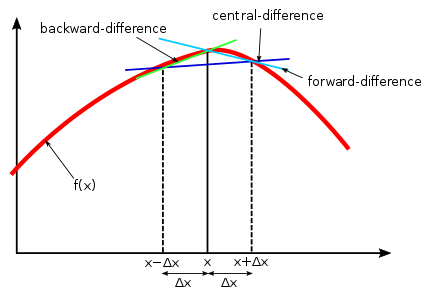
\includegraphics[width=110mm]{images/differencing.png}
  \caption{Visual illustration of differencing schemes\\ \cite{wiki:finiteDifference}}
  \label{fig:differencingschemes}
\end{figure}
In Figure \ref{fig:differencingschemes}, a visual representation of the differences between the approximation schemes is shown on a generic function taken as an example.
It is possible to see how the result of the approximation depends on the choice of $\Delta x_i$.
In particular, a step in the positive or negative direction can be taken, as well as in both of those. Respectively, these choices lead to forward, backward and central differencing method. \cite{masching_dissertation} \\[6pt]
Later on, it will be explained how the choice of the differencing scheme affects the results of the analysis.







	%%%%%%%%%%%%%%%%%%%%%%%%%%%%%%%%%%%%%%%%%%%%%%%%%%
%% Authors :    Giovanni Arcari                 %%
%%              Maria Bronzova                  %%
%%              Luca Sardi                      %%
%%              Spencer Sharp                   %%
%%                                              %%
%% Supervisor : Andreas Apostolatos             %%
%%											  	%%
%% e-mail : andreas.apostolatos@tum.de		   	%%
%%											  	%%
%% 03_Objective_functions.tex					%%
%%											  	%%
%%%%%%%%%%%%%%%%%%%%%%%%%%%%%%%%%%%%%%%%%%%%%%%%%%
\section{OBJECTIVE FUNCTIONS FOR SENSITIVITY ANALYSIS} \label{section:ObjectiveFunctions}
As previously anticipated, in general sensitivity analysis investigates the influence of a given perturbation on the input variables on the results. Connecting those two are the objective functions. \\[3pt]
Since the problem concerns a structural analysis, the objective functions which are taken into account are \textit{displacements}, \textit{strain energy} and \textit{Von Mises stress}.\\[3pt]
The results can be combined at the end in order to achieve what sensitivity analysis is particularly suitable for: optimization. \\[3pt]
For example, if the intent is to minimize displacements for a specific node, a sensitivity analysis will reveal which parts of the structure influence more heavily that node's displacement, and which parts have little influence. That would allow, for instance, to know where to stiffen the structure in order to get a lower displacement where desired. \\[3pt]
In the following sections, the different objective functions are illustrated, together with their derivation.

\subsection{Displacement}

From \cite{masching_dissertation}, adjoint variable for displacement sensitivity:
\begin{equation}
\Lambda = \textbf{K}^{-1}\cdot\textbf{v}
\label{}
\end{equation}

where...
\begin{equation}
\textbf{v}^T=[0 ...0\,\,1\,\,0...0]
\label{}
\end{equation}

Displacement sensitivity: 
\begin{equation}
\dv{D_{lin}}{s_i} = \Big[\pdv{\textbf{f}_{ext}}{s_i} - \pdv{\textbf{K}}{s_i} \cdot\textbf{u}\Big]^T \cdot \Lambda
\label{}
\end{equation}

\subsection{Strain energy}

From \cite{masching_dissertation}, adjoint variable for strain energy sensitivity:
\begin{equation}
\Lambda = \textbf{K}^{-1} \cdot \Big[\frac{1}{2}\cdot\textbf{f}_{ext} \Big] = \frac{1}{2}\textbf{u}
\end{equation}

where...
\begin{equation}
    \textbf{K}^{-1} = \big[ \pdv{\textbf{s}}{\textbf{u}}\big]
\end{equation}

and...
\begin{equation}
    \frac{1}{2}\cdot\textbf{f}_{ext} = \pdv{E_{lin}}{\textbf{u}}
\end{equation}
%$\textbf{K}^{-1} = \big[ \pdv{\textbf{s}}{\textbf{u}}\big]$ and %$\frac{1}{2}\cdot\textbf{f}_{ext} = \pdv{E_{lin}}{\textbf{u}}$ FIX\\[5pt]
Strain energy sensitivity:
\begin{equation}
\dv{E_{lin}}{s_i} = \frac{1}{2}\cdot\textbf{u}^T\cdot\pdv{\textbf{f}_{ext}}{s_i}+\Big[\pdv{\textbf{f}_{ext}}{s_i} - \pdv{\textbf{K}}{s_i} \cdot\textbf{u}\Big]^T \cdot \Lambda
\label{}
\end{equation}
\subsection{Von Mises stress}
From \cite{vonMises}, generally the von Mises stress expressed in principal stresses in 3D reads: 
\begin{equation} \label{eqn:vonMises3D}
\sigma^2_{von Mises}=\frac{1}{2}\big [\big(\sigma_{1}-\sigma_{2}\big )^2+\big(\sigma_{2}-\sigma_{3}\big )^2+\big(\sigma_{3}-\sigma_{1}\big )^2\big]
\end{equation}
For 2D problems, equation \ref{eqn:vonMises3D} can be simplified to equation \ref{eqn:vonMises2D}, which is what was used for the purpose of this assignment.
\begin{equation} \label{eqn:vonMises2D}
\sigma^2_{von Mises}=\sigma_{1}^2+\sigma_{2}^2-\sigma_{1}\cdot\sigma_{2}
\end{equation}
As the von Mises stress was treated only in the framework of the global sensitivity analysis, no further derivations for the adjoint sensitivity analysis have been made.
	
	%%%%%%%%%%%%%%%%%%%%%%%%%%%%%%%%%%%%%%%%%%%%%%%%%%%%
%%											  	 %%
%% Author : Andreas Apostolatos               	 %%
%%											  	 %%
%% e-mail : andreas.apostolatos@tum.de		   	 %%
%%											  	 %%
%% 04_Workflow.tex					  	   	 	 %%
%%											  	 %%
%%%%%%%%%%%%%%%%%%%%%%%%%%%%%%%%%%%%%%%%%%%%%%%%%%%%

\section{Workflow}
The framework for the analysis has been given by the Chair of Structural Analysis. In the following sections, a deeper look at each step of the analysis is taken. The software and codes are analyzed and discussed; the modification are illustrated, as well as the final code capabilities. 
\subsection{GiD}
%Fonte_ GiD website
GiD is an open source pre- and post-processor for numerical simulation in science and engineering, designed to cover some common needs in the numerical simulation field, such as: 
\begin{itemize}
\item Geometrical modeling (CAD) 
\item Mesh generation
\item Definition of analysis data
\item Data transfer to analysis software
\item Postprocessing operations
\item Result visualization
\end{itemize}
For the purpose of the assignment, just a few of the previously listed functions are used: thanks to GiD, a case to analyze is set, in terms of \textit{shape}, \textit{boundary conditions}, \textit{load case}. \\[6pt]
After that, a mesh is generated, and material law and mesh element type are assigned to the structure. \\[6pt]
The output of the illustrated procedure consists of a \texttt{.dat} text file, which can be taken as an input by the Matlab code. The \texttt{.dat} file contains all necessary aforementioned information.\\[6pt]
In order to improve the user experience, it was decided that expanding the GiD interface was preferred over hard coding sensitivity analysis information into Matlab. First of all, the given code was not able to deal with point loads. The first modification was to create an option for point loads application. The parser in Matlab was then modified accordingly to recognize and properly apply point loads to the given structure.\\[6pt]
In addition, a menu was created, such that the user has the possibility to customize the sensitivity analysis in different ways. In particular, choices are given with respect to: 
\begin {itemize}
\item \textbf{Method}: global, numerical adjoint or analytical adjoint
\item \textbf{Objective Function}: strain energy, displacement, Von Mises stress with node/element selection
\item \textbf{Differencing Scheme}: forward, backward, or central differencing
\end{itemize}
\subsection{Matlab}
In this paragraph, a brief explanation of the Matlab processing is given. For the purpose of the paper, it is thought that a qualitative discussion is sufficient, so no lines of code are included here, since it would be extremely complicated to write them in comprehensible, synthetic and significant way. The whole processing of the sensitivity analysis is done thanks to a code written in Matlab. The basis for that, as previously said, was given by the Chair of Structural Analysis.\\[6pt]
In particular, the parsers were already able to perform structural calculations, as the response function of a given structure subject to an assigned line load. \\[6pt]
First of all, for the sake of generality and completeness, the parsers were modified so that it is possible to assign a point load, an eventuality which was thought to be useful.\\[6pt]
Then, the different sensitivity analysis for the objective functions were developed. Basically, the implementation required to translate into the Matlab code the derivation which was shown in the theoretical background section. 

%Add which one is done with which method
\subsection{ParaView}
ParaView is an open source platform for interactive scientific visualization. Its only purpose in the given framework is to allow to get visual plots of the results. Here it is possible to see the structure, together with the mesh, the loads and the boundary conditions, and its response to the variation of the input variables. 



	%%%%%%%%%%%%%%%%%%%%%%%%%%%%%%%%%%%%%%%%%%%%%%%%%%%%
%%											  	 %%
%% Author : Andreas Apostolatos               	 %%
%%											  	 %%
%% e-mail : andreas.apostolatos@tum.de		   	 %%
%%											  	 %%
%% 05_Perturbation_study.tex					 %%
%%											  	 %%
%%%%%%%%%%%%%%%%%%%%%%%%%%%%%%%%%%%%%%%%%%%%%%%%%%%%

\section{Perturbation study} \label{section:perturbationstudy}
As shown throughout the previous sections, results in sensitivity analysis are also driven by the chosen value for the perturbation, which is used to approximate the derivatives in the finite differencing schemes.\\[6pt]
The aim of this section is to try to show the general error behavior, to make the reader conscious of how the simulation can be badly affected if the perturbation value is chosen without any attention.
\subsection{Error assessment for decreasing perturbation values}
First of all, for the sake of clarity, it's important to state what is meant by perturbation value: in fact, this represents the displacement of a node normalized by the length of the element in the accounted direction.\\[6pt]
It's important to remind how the value shown are related to the run analysis and don't hold for any case, and how the aim of the perturbation study is to show a generic trend. \\[6pt]
Here follows the procedure used to assess the error: first of all, a type of sensitivity analysis was chosen. In this case a displacement sensitivity was run first, later it was verified how the behavior - with different error value but a similar trend - holds for all the other analysis. \\[6pt]
Then, the value of the sensitivity at a designated node was taken and stored, the perturbation value changed and the analysis performed again. \\[6pt]
As error, the difference between the sensitivity from each analysis and the value to which it converged for decreasing values of perturbation is taken. The latter was deliberately rounded off in order not to have an exact zero value for the error, which could be misleading.\\[6pt]
Two differencing schemes - backward and central - are chosen.
By running the analysis, it was possible to get the following data, plotted here in a double logarithmic scale.
\begin{figure}[h]
\centering
  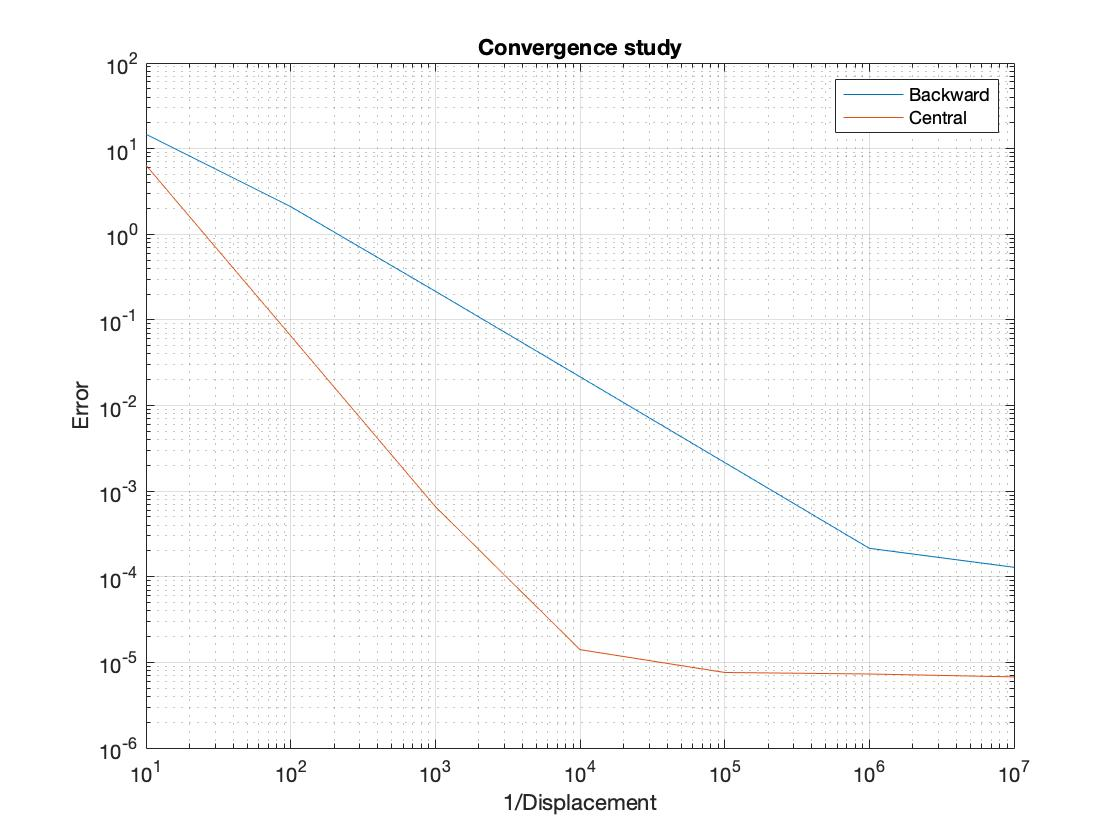
\includegraphics[width=140mm]{images/perturbation.jpg}
  \caption{Error assessment for decreasing perturbation values}
\end{figure}
\\[4pt] From this graph, it is possible to deduce some interesting information: first of all, the error decreases with twice the slope - in double logarithmic scale - for central differencing compared to backward and forward schemes, whose curve would overlap if both plotted. Then, it's noticeable how after a certain value, decreasing the perturbation does not lead to any change in the error: this is the range where a proper perturbation value can be chosen. \\[6pt]
Going further, it would be possible to see how the simulation blows up for perturbation value whose order of magnitude is around $10e-12$. This is due to the fact that the calculators are not able to represent any number, so at a certain level the results would just contain numerical waste.
	
	%%%%%%%%%%%%%%%%%%%%%%%%%%%%%%%%%%%%%%%%%%%%%%%%%%%%
%%											  	 %%
%% Author : Andreas Apostolatos               	 %%
%%											  	 %%
%% e-mail : andreas.apostolatos@tum.de		   	 %%
%%											  	 %%
%% 06_Problem.tex					  	   	 	 %%
%%											  	 %%
%%%%%%%%%%%%%%%%%%%%%%%%%%%%%%%%%%%%%%%%%%%%%%%%%%%%

\section{Problem case}

In order to show the capabilities of the code which has been developed, how results are shown, and how to interpret a sensitivity analysis, an example is provided.\\[6pt]
It's important to notice that the following constitutes just a single application of the code, which - as explained later - is able to perform calculations on any kind of arbitrary structure that the user sets up through GiD. In this particular case, the aim is to show a simple case, whose behavior can be found intuitive by those readers who have even just a basic understanding of structural mechanics.

\subsection{Sensitivity analysis on a cantilever beam}
\subsubsection{Geometry and boundary conditions}
As explained, the case for the analysis example is chosen to be intuitive and broadly known. For this reason, a cantilever beam has been chosen. As illustrated in Figure \ref{cantileverBeam:BCs}, the left edge of the beam is fixed; horizontal and vertical displacements are constrained, as well as the rotations.\\
\begin{figure}[ht]
\centering
  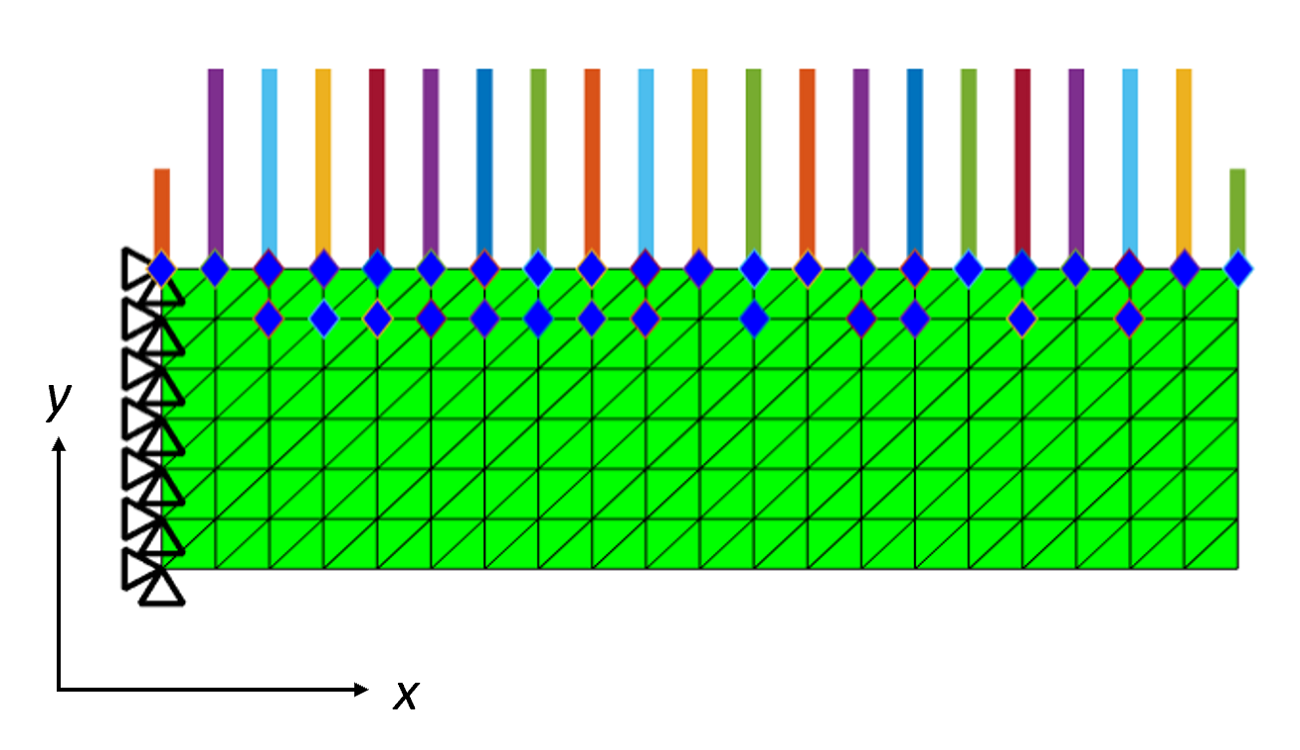
\includegraphics[width=100mm]{images/cantileverBeamBCs.png}
  \caption{Boundary conditions for cantilever beam}
  \label{cantileverBeam:BCs}
\end{figure} \\
The simulated beam has a width of $1.75m$ and a height of $0.5m$.
The slenderness, defined in this case by the ratio between the major and the minor dimensions, is  $3.5$. 
\subsubsection{Material properties}
In this example, the beam is made of steel.\\[6pt]
Accordingly, the following material properties have been applied to the model: 
\begin{itemize}
\item Young's modulus: $E = 210 GPa$
\item Poisson's ratio: $\nu = 0.33$
\item Thermal expansion coefficient: $\alpha = 0$
%\item Density: $\rho = has it been considered?$ MAYBE ADD LATER
\item Plane stress
\item Linear elastic isotropic
\end{itemize}
\subsubsection{Loads}
Loads have been applied on the upper edge, a constant pressure $p = 1x10^{3} \frac{N}{m}$ in the negative y-direction is considered.
%[ADD IMAGE]
\subsubsection{Mesh}
%[ADD IMAGE AND COMMENTS]
GiD provides the user with various options for mesh generation. For the purpose of this example, a simple structured mesh consisting of linear triangular elements has been created using GiD's automatic mesh generation function. See Figure \ref{cantileverBeam:mesh} below. \\[6pt]
According to finite element literature, the number of element should be the smallest which can capture the behavior of the structure to a satisfying extent, in order to get good results and reasonable computational effort. \\[6pt] %NEED TO CITE THIS
As noticed by running different cases, it is possible to get a non-distorted mesh by choosing this length as an integer fraction of the beam dimension. Since the structure is rectangular, it is possible to get a uniform mesh, where all triangles have the same shape and size, and no distortion occurs. \\

\begin{figure}[ht]
\centering
  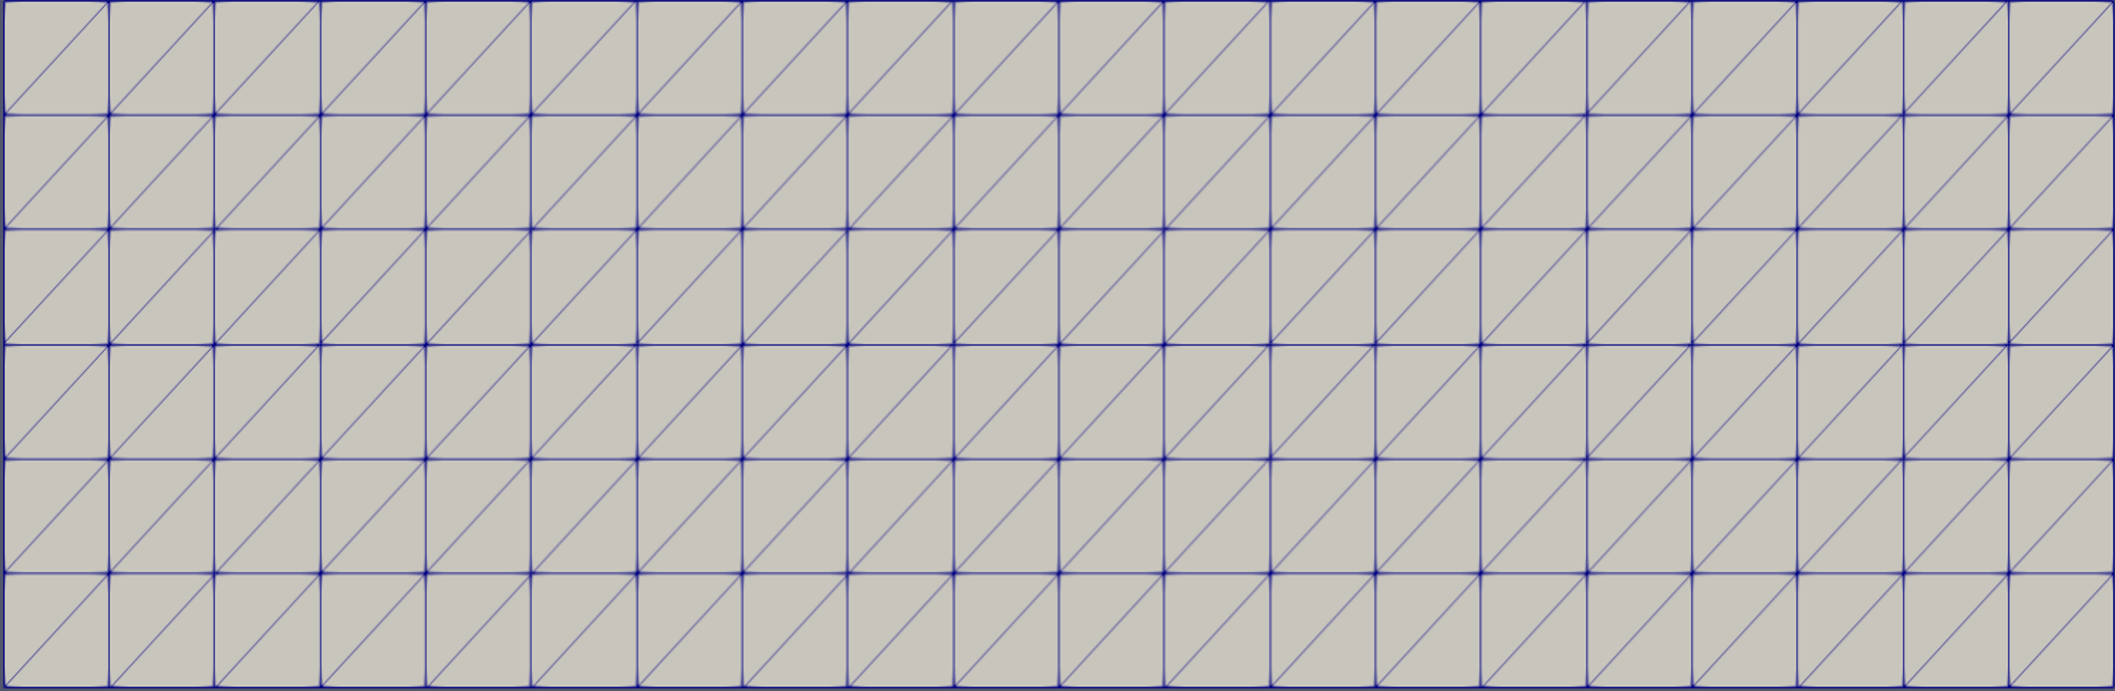
\includegraphics[width=100mm]{images/mesh.png}
  \caption{Generated mesh for cantilever beam}
  \label{cantileverBeam:mesh}
\end{figure}
In this case, six elements are chosen in the vertical direction, and 20 in the horizontal direction. Since the mesh is triangular, this leads to a total of 240 elements. It could be argued that the mesh is even too fine for the problem case; however, it's useful to keep in mind that the computational time using a common laptop was short enough to that no significant advantage could be had by the usage of a coarser mesh. Therefore, the mesh is kept as shown in the figure.\\[6pt]
For the purpose of numerical integration over both the domain and the boundary, the number of Gauss points must be specified. GiD defaults to assuming one Gauss point per element, which is what was used in this example.\\[6pt]



	%\newpage
	
	%%%%%%%%%%%%%%%%%%%%%%%%%%%%%%%%%%%%%%%%%%%%%%%%%%%%
%%											  	 %%
%% Author : Andreas Apostolatos               	 %%
%%											  	 %%
%% e-mail : andreas.apostolatos@tum.de		   	 %%
%%											  	 %%
%% 07_Results.tex					  	   	 	 %%
%%											  	 %%
%%%%%%%%%%%%%%%%%%%%%%%%%%%%%%%%%%%%%%%%%%%%%%%%%%%%

\section{Results}

\subsection{Displacement sensitivity}

Since the displacement sensitivity has a local meaning, a node has to be selected within the mesh, where the analysis is request to be performed. In this case, node 144 - circled in red in figure \ref{cantileverBeam:nodeOfInterest} below - has been chosen. It is situated in the middle of the free end of the cantilever beam. \\
\begin{figure}[ht]
\centering
  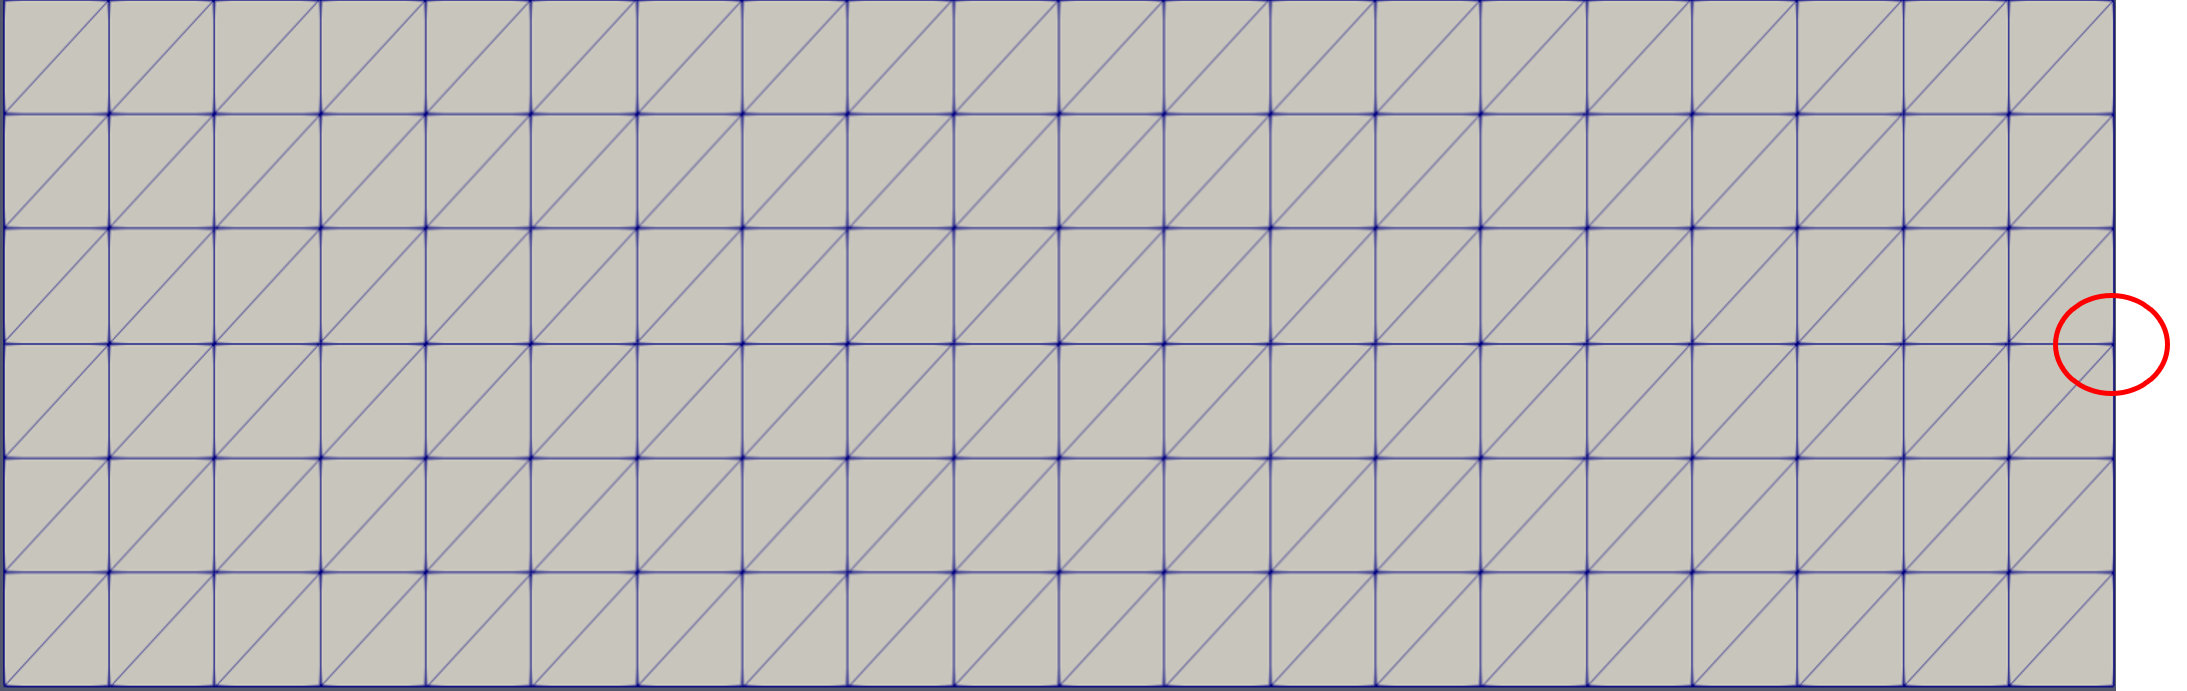
\includegraphics[width=100mm]{images/meshNodeOfInterest.png}
  \caption{Node 144}
  \label{cantileverBeam:nodeOfInterest}
\end{figure}\\
Since the perturbation is performed separately in $x$ and $y$ direction, two different plots are shown below, in order to clearly represent which influence is due to which perturbation. \\
\begin{figure}[ht]
\centering
\begin{minipage}{.5\textwidth}
  \centering
  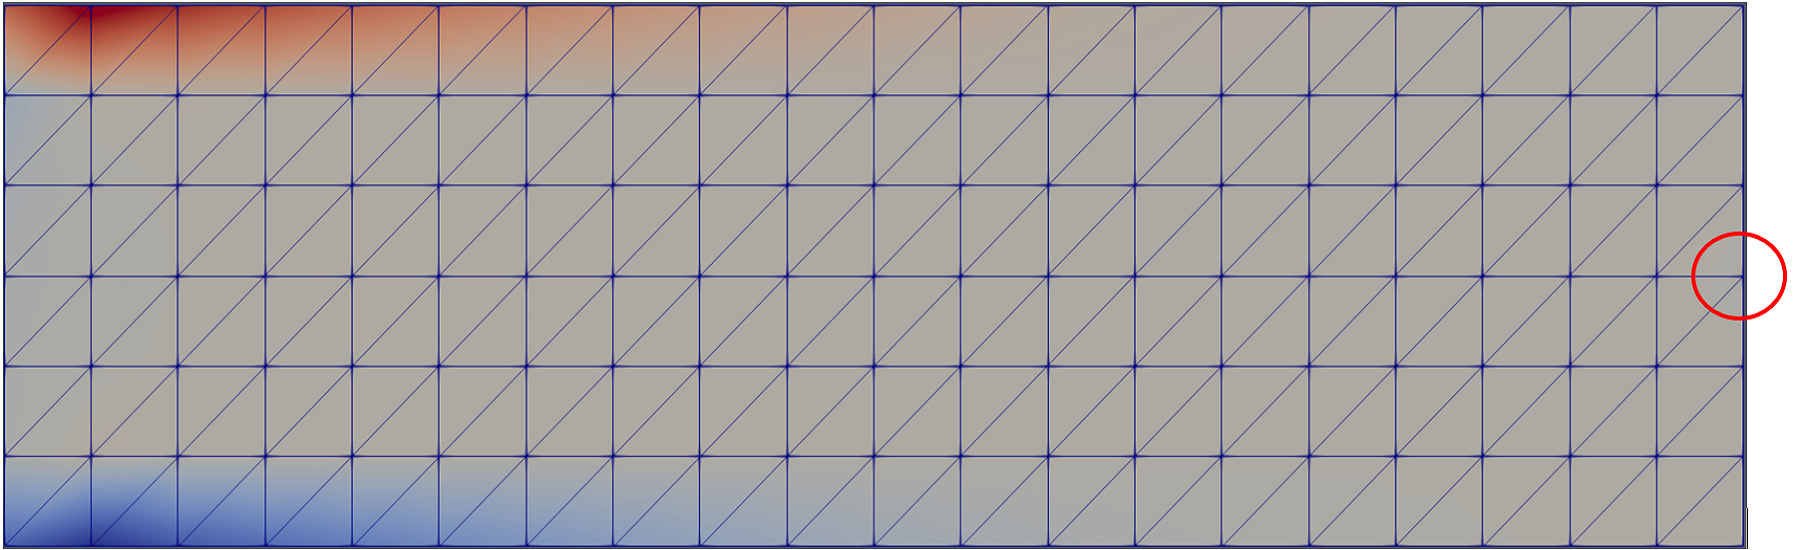
\includegraphics[width=1.0\linewidth]{images/sensitivityanalysisY.png}
  \captionof{figure}{displacement sensitivity, y-perturbation}
  \label{fig:yDispSens}
\end{minipage}%
\begin{minipage}{.5\textwidth}
  \centering
  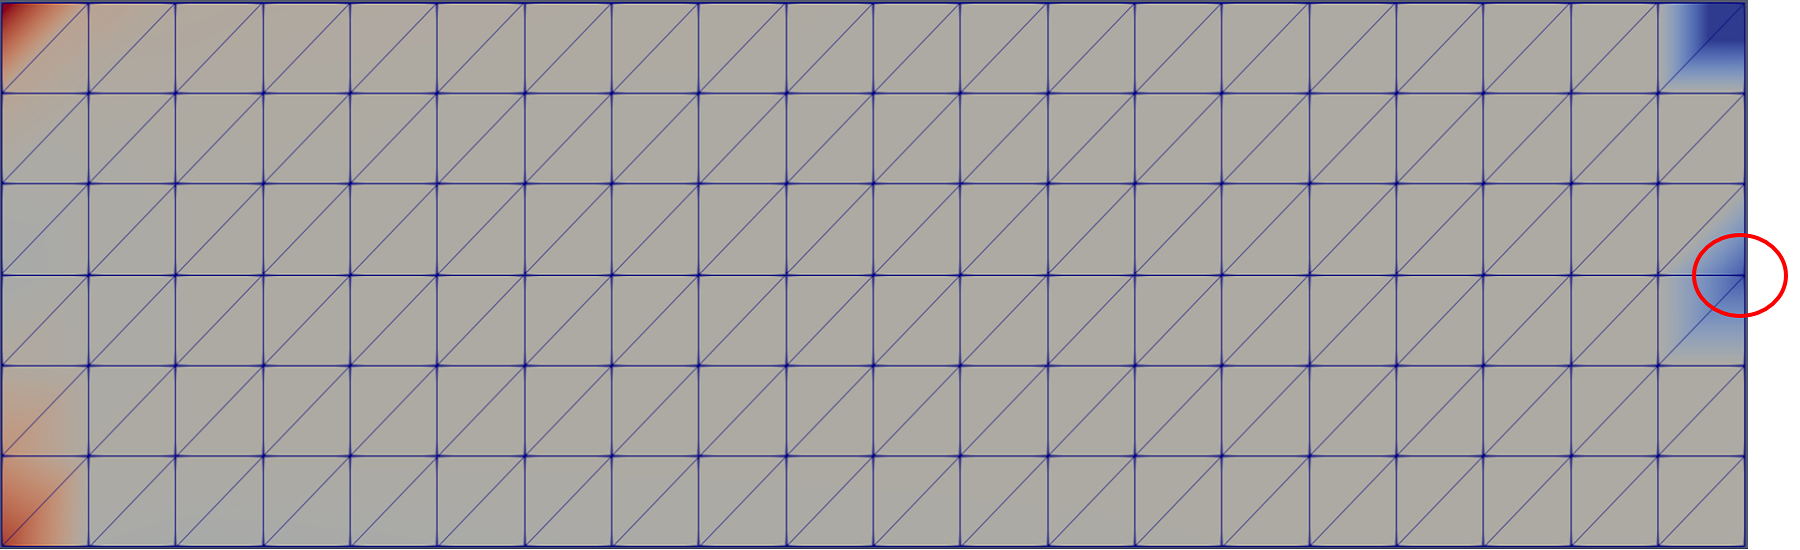
\includegraphics[width=1.0\linewidth]{images/sensitivityanalysisX.png}
  \captionof{figure}{displacement sensitivity, x-perturbation}
  \label{fig:xDispSens}
\end{minipage}
\end{figure}\\
With these plots, a first interpretation of the analysis can be done. Intensely colored blue and red areas represent parts of the structure where a displacement of that area affects the most the displacement of node 144. \\[6pt]
Figure \ref{fig:yDispSens}, which represents the sensitivity of node 144 with respect to a perturbation of all nodes in the upward $y$-direction, is probably the more intuitive to interpret. The nodes in the upper left portion of the beam are colored red. Displacing these nodes in the upward direction effectively increases the cross sectional area of the beam. Given that this is a cantilever beam, the cross sectional area at the clamped end has the largest influence on the displacement at the free end. Therefore, displacing the upper left nodes upward increases the stiffness of the beam and reduces the displacement of node 144. Accordingly, the nodes at the bottom left of the beam reduce the cross sectional area, thereby increasing the displacement of node 144. Hence, they are colored blue.\\[6pt]
Figure \ref{fig:xDispSens} represents the sensitivity of node 144 with respect to a perturbation of all nodes in the positive $x$ (right-ward) direction. Based on the plot, displacement of the nodes in the upper left and bottom left results in lower displacement of node 144. Modifying the length of the upper surface of the beam influences the total loading. Displacing the upper left node to the right effectively reduces the length of the upper surface, thereby reducing the loading. This reduces the displacement at node 144. Displacing the upper right node to the right has the opposite effect.\\[6pt]
Further comments will be provided in the optimization section, \ref{section:optimization}.

\subsection{Strain energy sensitivity} \label{section:strainSens}
In contrast to the displacement sensitivity, the strain energy sensitivity is inherently a global value. It represents the energy of a system undergoing deformation. Equation \ref{eqn:strainenergy} from \cite{wiki:strainEnergy} below describes strain energy for a linear elastic material.\\
\begin{equation} \label{eqn:strainenergy}
U = \frac{1}{2}V\sigma\epsilon
\end{equation}\\
Where $V$ represents the volume of the structure, $\sigma$ represents stress, and $\epsilon$ represents strain. Since the energy of the structure is global, a node does not need to be chosen; the analysis is performed on the entire structure. Figure \ref{fig:ystrainDispSens} and Figure \ref{fig:xstrainDispSens} below illustrate the effect on the strain energy of perturbing all nodes in the y-direction and all nodes in the x-direction, respectively. \\
\begin{figure}[ht]
\centering
\begin{minipage}{.5\textwidth}
  \centering
  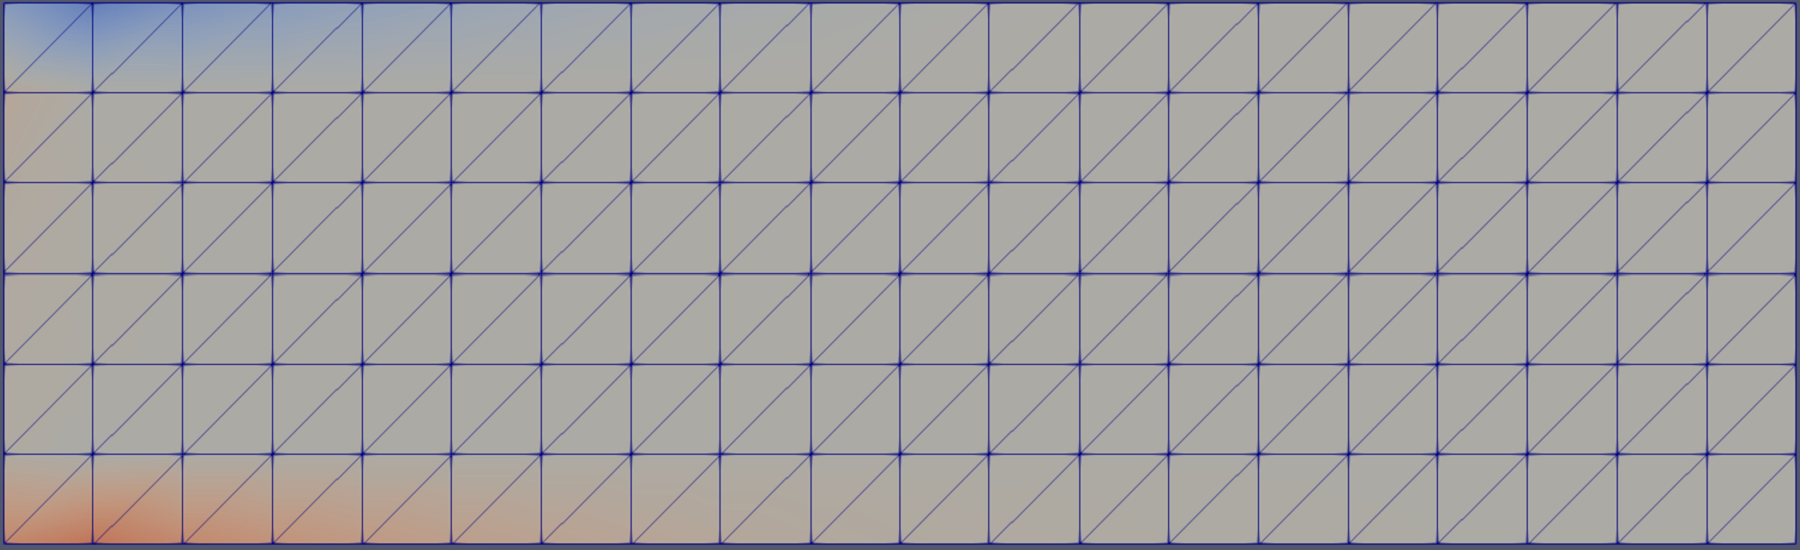
\includegraphics[width=0.95\linewidth]{images/strainsensitivityanalysisY.png}
  \captionof{figure}{strain energy sensitivity, y-perturbation}
  \label{fig:ystrainDispSens}
\end{minipage}%
\begin{minipage}{.5\textwidth}
  \centering
  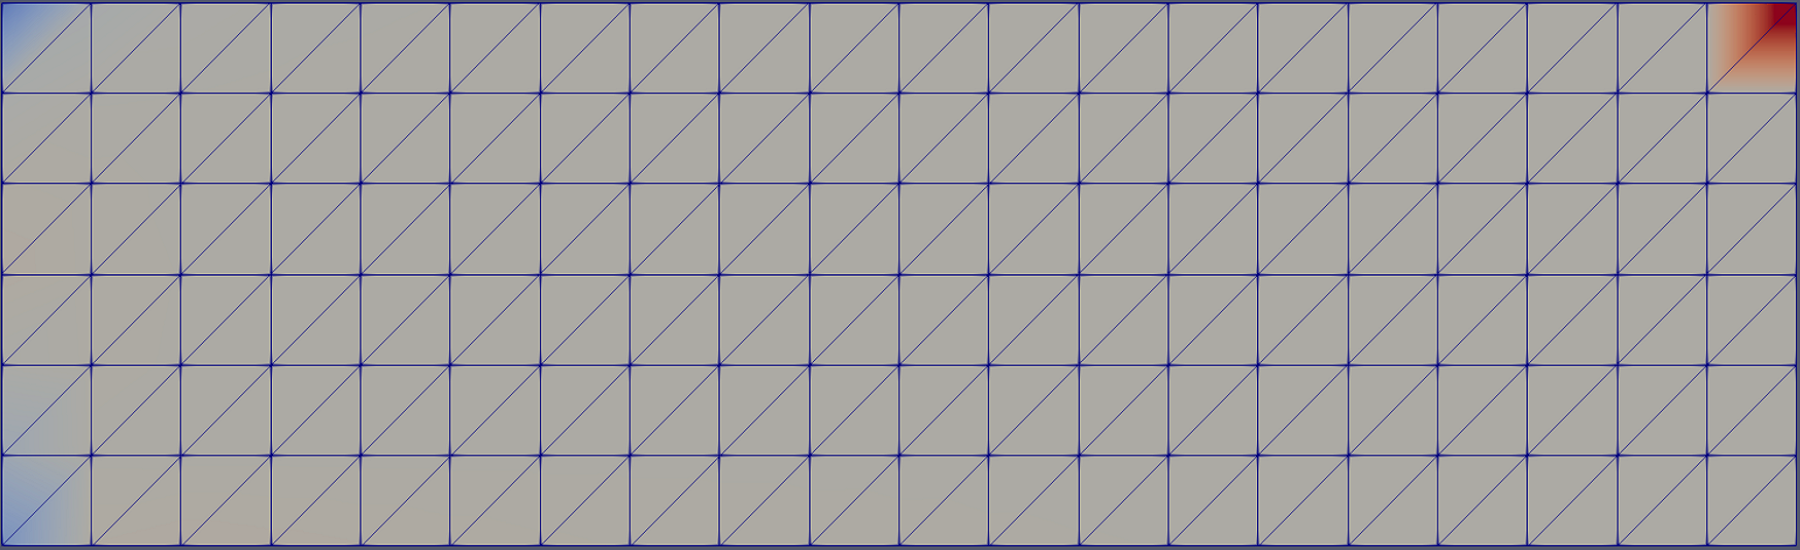
\includegraphics[width=0.95\linewidth]{images/strainsensitivityanalysisX.png}
  \captionof{figure}{strain energy sensitivity, x-perturbation}
  \label{fig:xstrainDispSens}
\end{minipage}
\end{figure}\\
In Figure \ref{fig:ystrainDispSens} above, one could make interpretations similar to those of Figure \ref{fig:yDispSens} in the previous section. In this case, the strain energy sensitivity is a function of volume, stress, and strain. The y-perturbation of nodes in the upper left and bottom right of the beam have the largest impact on the overall strain of the structure, which influences the strain energy the most. These results are very similar to those illustrated in Figure \ref{fig:yDispSens} because both simulations involve strain, which is related to displacement.\\[6pt]
Thus, it follows that the results of Figure \ref{fig:xstrainDispSens} mirror those of Figure \ref{fig:xDispSens} since the x-perturbation of the nodes along the top surface will influence the loading, which affects the overall strain energy.

\subsection{Optimization} \label{section:optimization}
Sensitivity analysis allows one to understand which parts of the structure affect most, for example, the strain energy of the structure itself. Then, how can this approach be used for optimizing the structure? \\[6pt]
For the sake of consistency, consider again the cantilever beam example. An optimization exercise may involve finding a geometry which minimizes the strain energy of the structure.\\[6pt]
As illustrated by the sensitivity analysis, it is possible to identify the areas which affect the strain energy of the system the most. So, the structure optimization is performed as follows.
\begin{enumerate}
    \item A sensitivity analysis is performed for a specific objective function, based on user selection in GiD. If applicable, the user can select one or more node(s) or element(s)
    \item The nodal coordinates in x- and y-directions are updated by adding a particular factor found in equation \ref{eqn:nodalAdjustment} below
    \item Repeat steps 1. and 2. until desired number of iterations is reached
\end{enumerate}

\begin{equation} \label{eqn:nodalAdjustment}
    \textbf{x}_{new} = \textbf{x} + \textbf{nodalSensitivity} \cdot perturbation \cdot scalingFactor 
\end{equation}\\
As explained above, the sensitivity analysis forms the heart of the optimization algorithm. It essentially assigns a value to each node representing its effect on the objective function. Then, for each node, this sensitivity value is multiplied by the perturbation size to transform this value into a distance. Next, it is multiplied by a scaling factor to help avoid unstable behavior. Finally, it is added to the "old" nodal coordinate to form the new nodal coordinate. These steps are repeated until the maximum number of iterations, $n$, is reached. The final result is the optimized structure, which has a different shape than the starting one, and whose shape minimizes - in this case - the strain energy. \\[6pt]
Based on the results discussed in section \ref{section:strainSens}, the most sensitive areas of the structure are the upper right, upper left, and bottom left corners. Therefore, those are the areas targeted by the optimization algorithm. See Figures \ref{cantileverBeam:BCs2} and \ref{cantileverBeam:BCs2} below.\\
\begin{figure}[ht]
\centering
\begin{minipage}{.5\textwidth}
  \centering
  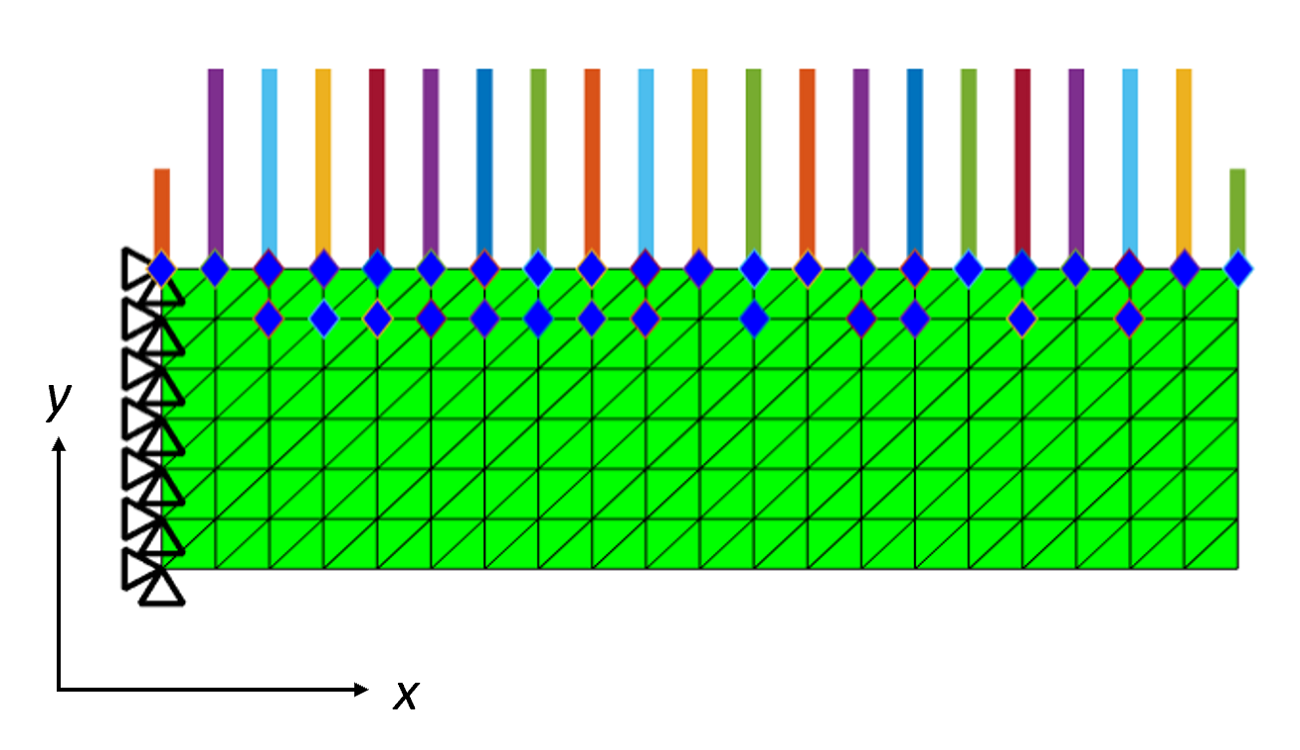
\includegraphics[width=1.0\linewidth]{images/cantileverBeamBCs.png}
  \captionof{figure}{cantilever beam, original geometry}
  \label{cantileverBeam:BCs2}
\end{minipage}%
\begin{minipage}{.5\textwidth}
  \centering
  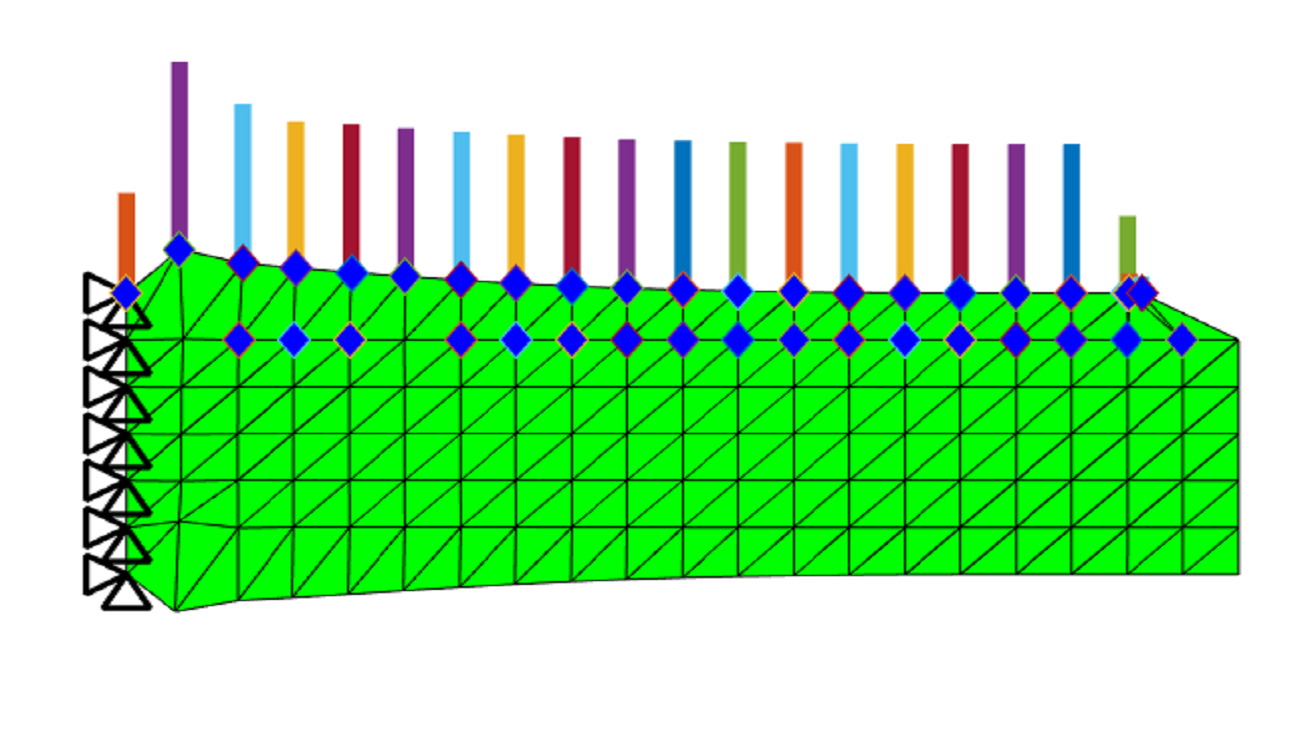
\includegraphics[width=1.0\linewidth]{images/cantileverBeamOptimized.png}
  \captionof{figure}{cantilever beam, optimized geometry}
  \label{fig:optimizedGeometry}
\end{minipage}
\end{figure}
After 10 iterations, a strain energy reduction of almost 54\% is achieved, without affecting heavily the shape of the beam. While this case considered only optimizing for strain energy, this optimization can be executed for any objective function.\\[6pt]
\begin{figure}[ht]
\centering
\begin{minipage}{.5\textwidth}
  \centering
  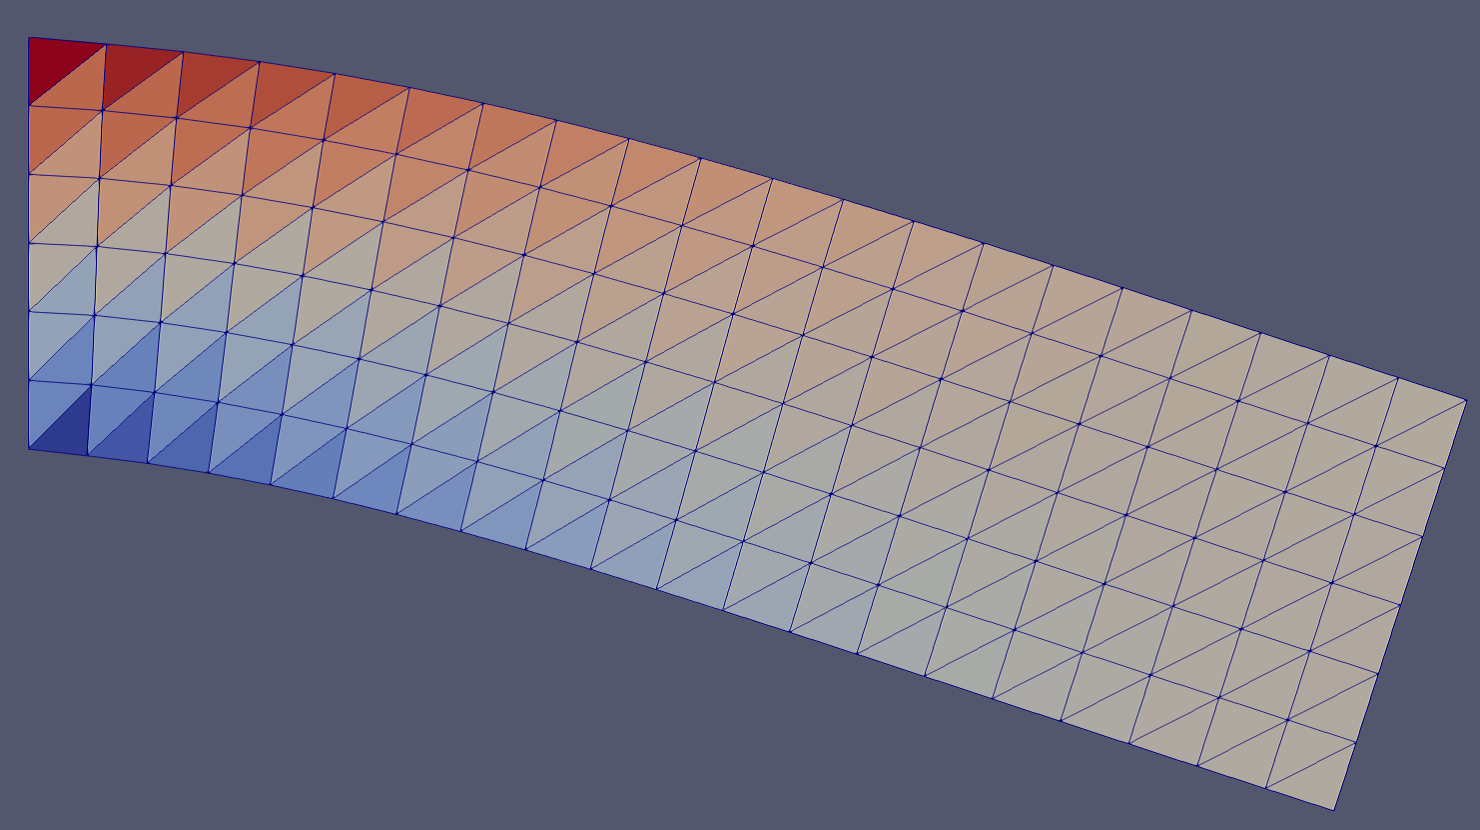
\includegraphics[width=0.9\linewidth]{images/strainAnalysis_original.png}
  \captionof{figure}{strain distribution, original geometry}
  \label{fig:strainAnalOrig}
\end{minipage}%
\begin{minipage}{.5\textwidth}
  \centering
  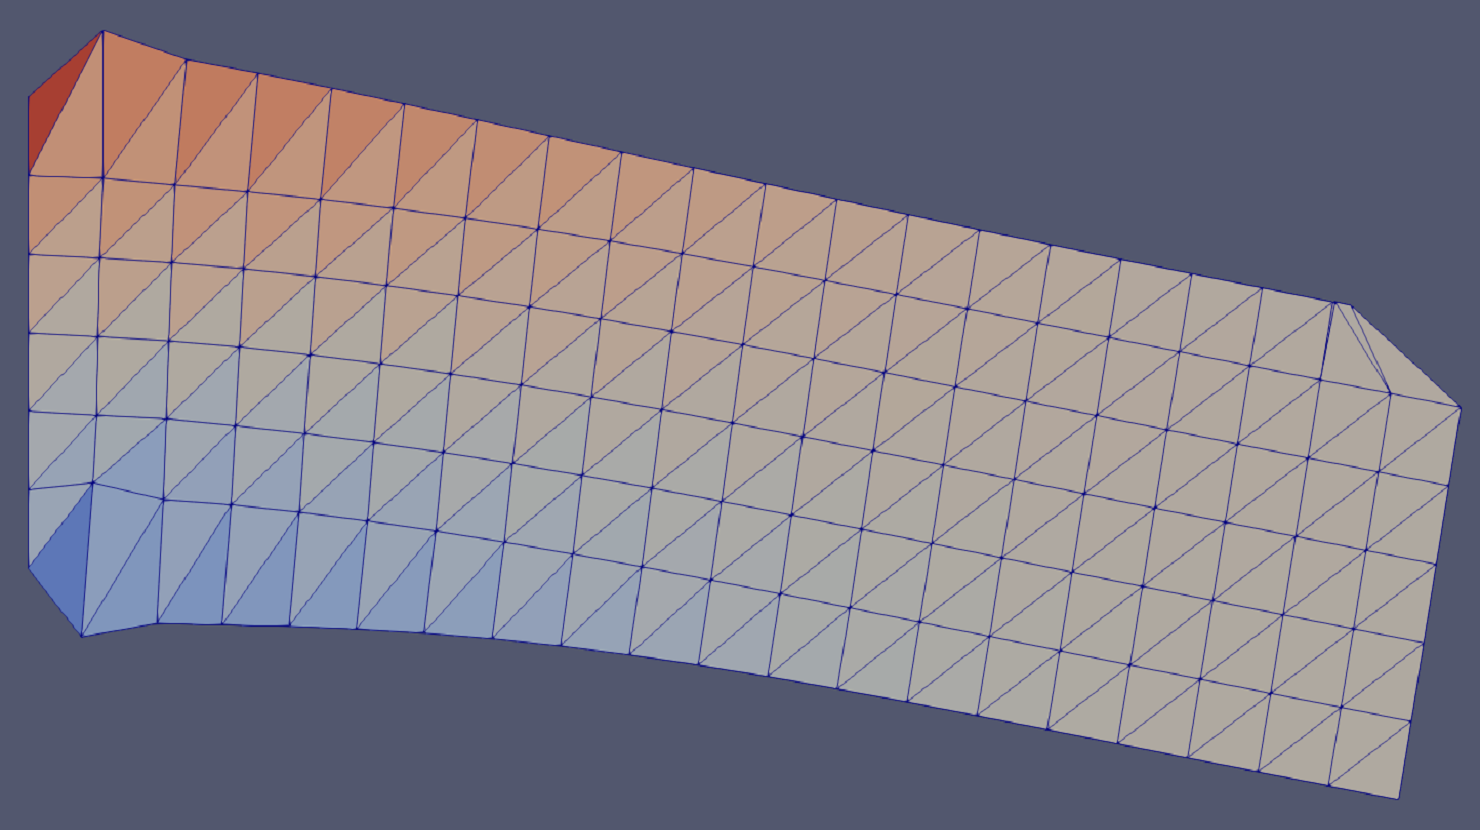
\includegraphics[width=0.9\linewidth]{images/strainAnalysis_optimized.png}
  \captionof{figure}{strain distribution, optimized geometry}
  \label{fig:strainAnalOpt}
\end{minipage}
\end{figure}
Figures \ref{fig:strainAnalOrig} and \ref{fig:strainAnalOpt} illustrate the stress distribution over the deformed cantilever beam in both the original and optimized geometry, respectively. Since the same color scale is used for both images, it is possible to qualitatively see that the strain has generally decreased from the original to the optimized geometry. This reduced strain, of course, contributes to the reduced strain energy previously mentioned.\\[6pt]
To generate this new, optimized geometry, the optimization algorithm iterated 10 times, which was predefined. This choice is primarily due to the fact that more iterations results in unstable behavior. This instability is due to the lack of an additional constraining equation. Often, multi-objective optimization is performed, whereby multiple objective functions are optimized. In this example, the algorithm would theoretically keep increasing the cross sectional area at the base, if it were not for the iteration limit. Of course, this is not realistic as engineers often want to minimize weight, volume, cost, etc. Therefore, a future improvement to this program would be to allow for optimizing multiple, opposing objective functions so that the algorithm can iterate until convergence is reached, rather than a maximum number of iterations.




	%\newpage
	
	%%%%%%%%%%%%%%%%%%%%%%%%%%%%%%%%%%%%%%%%%%%%%%%%%%%%
%%											  	 %%
%% Author : Andreas Apostolatos               	 %%
%%											  	 %%
%% e-mail : andreas.apostolatos@tum.de		   	 %%
%%											  	 %%
%% 08_Conclusions.tex					  	   	 %%
%%											  	 %%
%%%%%%%%%%%%%%%%%%%%%%%%%%%%%%%%%%%%%%%%%%%%%%%%%%%%

\section{Conclusions} %no more than one paragraph
Sensitivity analysis is a powerful tool in the field of Structural Design. In general, it quantifies the effect of input variables on output variables of an objective function. There are three basic categories of sensitivity analyses: global, semi-analytical, and analytical. All three were implemented in Matlab, utilizing the provided finite element code as a basis. Three different objective functions were implemented: strain energy, displacement, and Von Mises stress. In addition, the GiD user interface was enhanced to allow the user to input point loads, customize his/her desired sensitivity analysis, and input parameters needed for optimization. This information is passed fluidly to Matlab, where the implemented code will generate an output file that can be visualized in Paraview.

	
	%\newpage
	\nocite{*} %Even non-cited BibTeX-Entries will be shown.
	\printbibliography
	   
	%\newpage
	\appendix

    %%%%%%%%%%%%%%%%%%%%%%%%%%%%%%%%%%%%%%%%%%%%%%%%%%%%
%%											  	 %%
%% Author : Andreas Apostolatos               	 %%
%%											  	 %%
%% e-mail : andreas.apostolatos@tum.de		   	 %%
%%											  	 %%
%% 09_Appendix.tex					  	   	  	 %%
%%											  	 %%
%%%%%%%%%%%%%%%%%%%%%%%%%%%%%%%%%%%%%%%%%%%%%%%%%%%%
\section{Appendix}

Here all theorems or general concepts that have been used in the report and seek further explanation should be placed.\\[6pt]
Note that the references come before the appendix. The references need to be written in .bib format, see the attached file references.bib. Then you should compile three times the document with bibTex and other three times with LatexMk (or simply Latex) and they should normally appear into the text automatically.\\[6pt]
%%%%%%%%%%%%%%%%%%%%%%%%%%%%%% MATLAB %%%%%%%%%%%%%%%%%%%%%%%%%%%%%%%%
\subsection{Matlab Code} \label{section:appendix_matlab}
[INSERT CONTENT (AND SUBSECTIONS IF NEEDED)]

%%%%%%%%%%%%%%%%%%%%%%%%%%%%%%% GiD %%%%%%%%%%%%%%%%%%%%%%%%%%%%%%%%%%
\subsection{GiD GUI} \label{section:appendix_GiD}
The GiD user interface was modified as part of this assignment in order to facilitate the simple transfer of data from GiD to Matlab. All data entered by the user in GiD is contained within the \texttt{.dat} file generated by GiD. Matlab reads the \texttt{.dat} file as an input for the calculations. Please note that only the functionality

%%%%%%%%%%%%%%%%%%%%%%%%%%%% GiD - Setup %%%%%%%%%%%%%%%%%%%%%%%%%%%%%
\subsubsection{Setup}
GiD is equipped with various \texttt{problem types}, which contain the commands to customize the user interface. All of the enhancements made to GiD are within the \texttt{Matlab} problem type. To select this, under the \texttt{Data} heading, click \texttt{Problem type} $\rightarrow$ \texttt{matlab}. See Figure \ref{fig:Matlabproblemtype}.

\begin{figure}[ht]
  \centering
  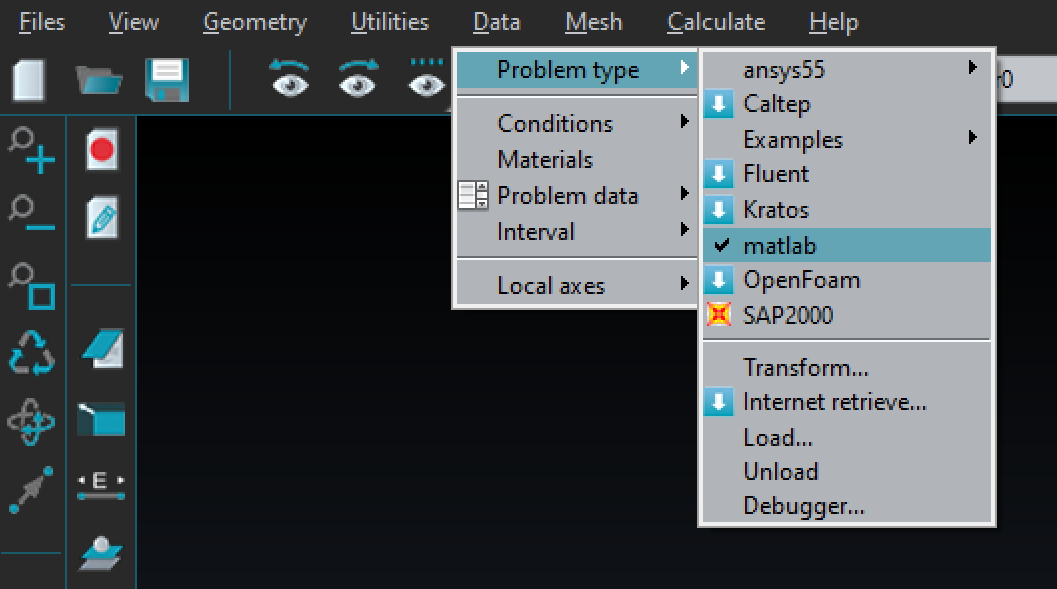
\includegraphics[width=80mm]{images/GiD_probtype.png}
  \caption{\texttt{Matlab} problem type selection}
  \label{fig:Matlabproblemtype}
\end{figure}
Next, create a geometry using the \texttt{geometry} $\rightarrow$ \texttt{create} menu.

%%%%%%%%%%%%%%%%%%%%%%% GiD - boundary conditions %%%%%%%%%%%%%%%%%%%%%%%%
\subsubsection{Boundary Conditions}
Once the geometry is created, the user must apply boundary conditions in order to constrain the model. Click \texttt{Data} $\rightarrow$ \texttt{Conditions} $\rightarrow$ \texttt{Constraints}, and the menu shown in Figure \ref{fig:GiDConstraints} will appear. For a plane stress problem, only $x$ and $y$ constraints should be applied. In the example shown in this paper, a value of 0.0 was used for each.\\[6pt]
\begin{figure}[ht]
  \centering
  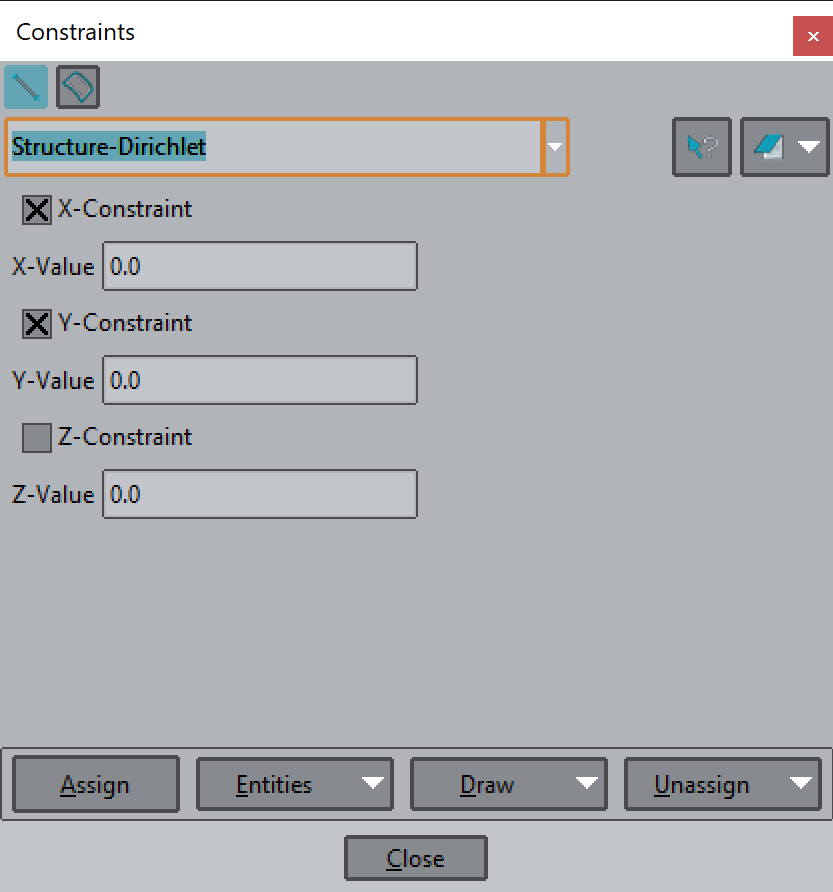
\includegraphics[width=60mm]{images/GiD_constraints.png}
  \caption{constraints menu}
  \label{fig:GiDConstraints}
\end{figure}
Next, click \texttt{Assign} and then click on the edge of the model to apply the desired constraint.

%%%%%%%%%%%%%%%%%%%%%%%%%%%%% GiD - loads %%%%%%%%%%%%%%%%%%%%%%%%%%%%%%%%%
\subsubsection{Loads}
The first modification made to GiD was to allow for the application of point loads. The primary purpose for this was to simplify equation \ref{eqn:responsefctderivative}. The term $\dv{\textbf{P}}{x_i}$ represents the change in the force vector, $\textbf{P}$, with respect to the design variables, $x_i$. This term vanishes if the force vector is constant with respect to the design variables, which is the case when a point load is applied. This simplified equation would make initial implementation and validation of the numerical and analytical sensitivity equations a bit easier\\[6pt]
The ability to apply a distributed load was already contained within the \texttt{Matlab} problem type. To apply a load, simply click on the \texttt{Data} heading, then \texttt{conditions} $\rightarrow$ \texttt{loads}. The menu shown in Figure \ref{fig:GiDLoadsDist} will appear. There are only two actions that need to be taken. First, select the proper function handle. There is a \texttt{computeConstantVerticalLoad} and a \texttt{computeConstantHorizontalLoad} option. They correspond to functions within the Matlab code hierarchy that assign a constant vertical or horizontal load, respectively. In these functions, the user can input the desired load magnitude. Second, click \texttt{Assign}. Then, select the edge of the structure on which to apply the distributed load.

\begin{figure}[ht]
  \centering
  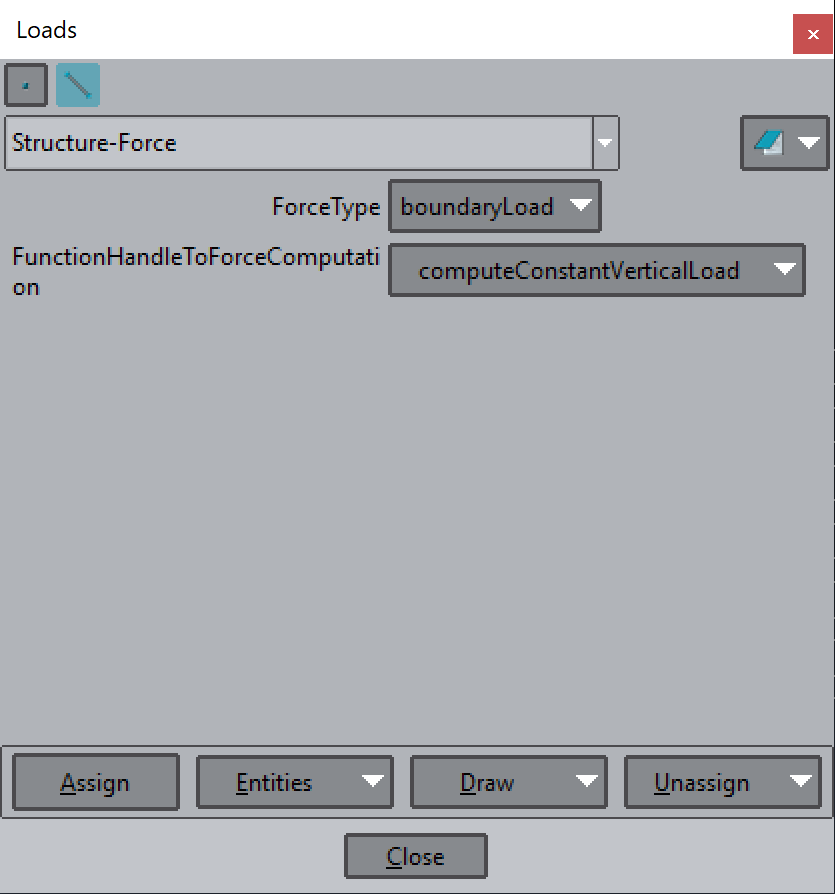
\includegraphics[width=60mm]{images/GiD_loads_dist.png}
  \caption{distributed loads menu}
  \label{fig:GiDLoadsDist}
\end{figure}

In addition to being able to apply a distributed load, the user can apply a point load. This is the functionality added to aid the development of the sensitivity analysis program. The associated menu is also under \texttt{Data} $\rightarrow$ \texttt{Conditions} $\rightarrow$ \texttt{Loads}. Simply click on the symbol in the upper left of the menu to toggle between point and distributed loads. See Figure \ref{fig:GiDLoadsPoint}. Before applying a point load, the mesh must first be generated! The most simple way to generate a mesh in GiD is to click \texttt{Mesh} $\rightarrow$ \texttt{Generate mesh}. Then, enter the desired element size. \textbf{Note:} too small of a mesh size will cause long calculation times.

\begin{figure}[ht]
  \centering
  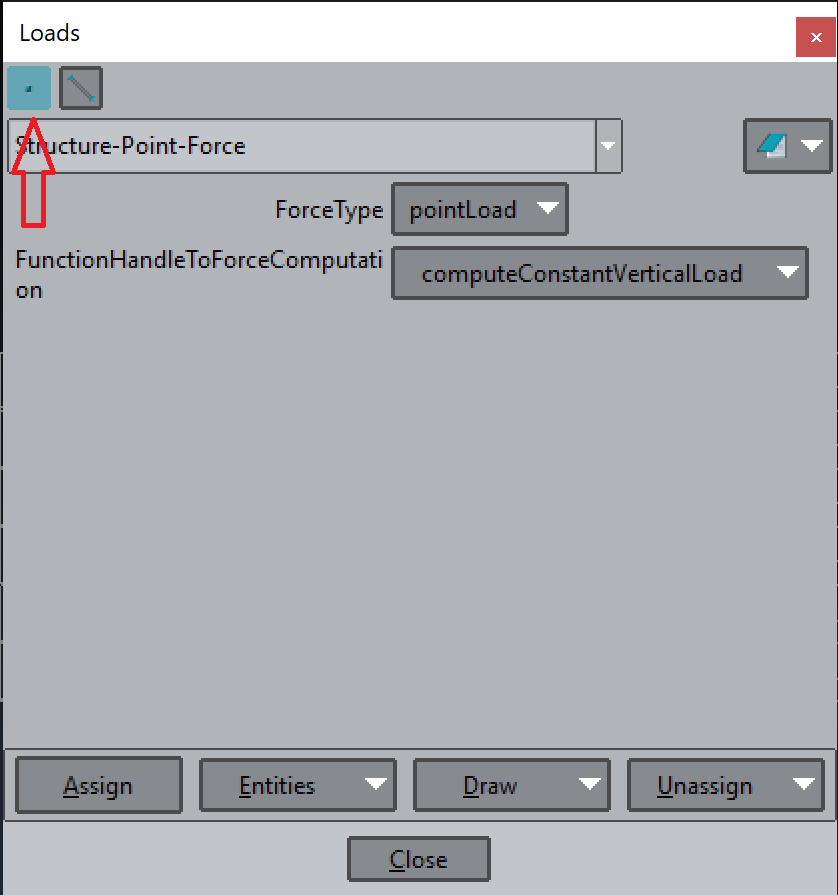
\includegraphics[width=60mm]{images/GiD_loads_point.png}
  \caption{point loads menu}
  \label{fig:GiDLoadsPoint}
\end{figure}
%%%%%%%%%%%%%%%%%%%%%%%% GiD - sensitivity analysis %%%%%%%%%%%%%%%%%%%%%%
\subsubsection{Sensitivity Analysis}
To define the sensitivity analysis parameters, click \texttt{Data} $\rightarrow$ \texttt{Problem Data} $\rightarrow$ \texttt{Sensitivity Analysis}. The menu shown in Figure \ref{fig:GiDSensAnalMenu} will appear. In the upper dropdown menu, the user can select the type of sensitivity analysis. The options are: \texttt{global}, \texttt{numerical adjoint}, and \texttt{analytical adjoint}. Exercise caution when selecting the global method - please ensure a relatively low number of nodes (less than ~200) is used. In the sensitivity analysis menu, the user can click the box next to the desired objective functions. Please note that currently, the von Mises stress objective function only works with the global method due to time constraints. Next, the user can select the finite differencing method: \texttt{forward}, \texttt{backward}, or \texttt{central}. Finally, the user can select the perturbation size. Based on the perturbation study discussed in section \ref{section:perturbationstudy}, a perturbation of $10^{-5}$ worked reliably.
\begin{figure}[ht]
  \centering
  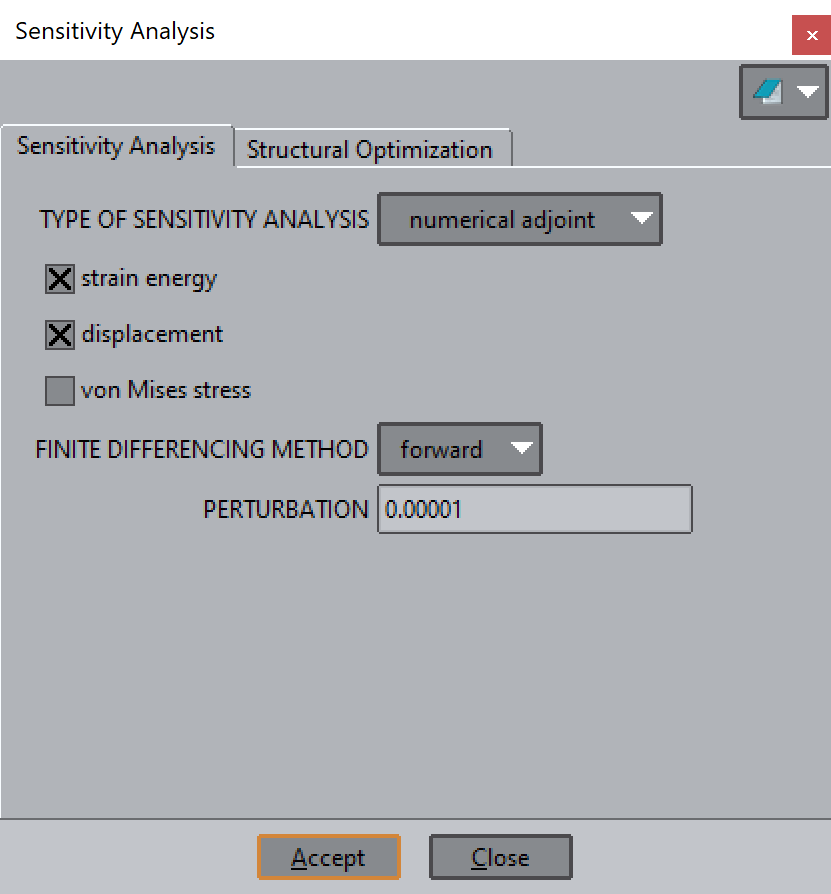
\includegraphics[width=60mm]{images/GiD_sens_analysis.png}
  \caption{sensitivity analysis menu}
  \label{fig:GiDSensAnalMenu}
\end{figure}

%%%%%%%%%%%%%%%%%%%%%%%%%%%% GiD - domains %%%%%%%%%%%%%%%%%%%%%%%%%
\subsubsection{Domains}
Next, click \texttt{Data} $\rightarrow$ \texttt{Conditions} $\rightarrow$ \texttt{Domains}. The menu shown in Figure \ref{fig:GiDDomainsMenu} will appear. In the dropdown menu, click \texttt{Structure-Nodes}, click \texttt{Assign}, select all nodes, and click \texttt{Finish}. Click \texttt{Structure-Elements} in the dropdown menu and perform the same steps.\\[6pt]
Next, parameters associated with the sensitivity analysis must be specified. These are also visible in Figure \ref{fig:GiDDomainsMenu} If a displacement sensitivity analysis is selected, then the user must specify which node(s) on which to perform the analysis. Simply click \texttt{Structure Nodes for Displacement Sensitivity}, \texttt{Assign}, and then select the appropriate node(s). The same steps apply to von Mises stress, except the user must select one or more elements instead of nodes. For a strain energy sensitivity analysis, no further action is needed since the analysis is applicable to the entire structure.
\begin{figure}[ht]
  \centering
  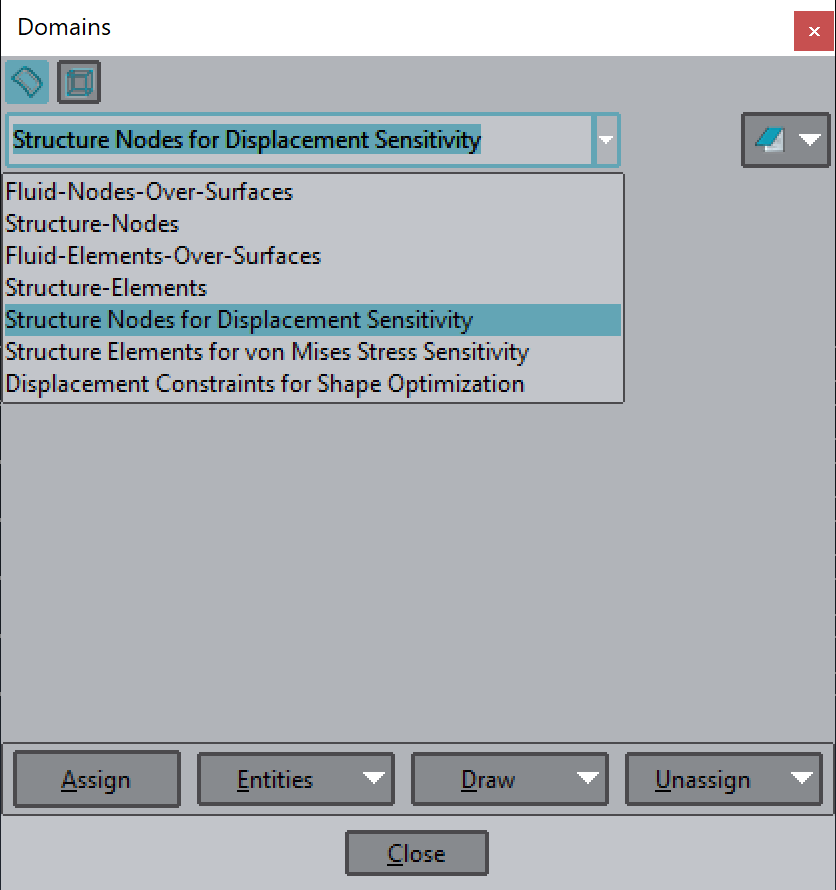
\includegraphics[width=60mm]{images/GiD_domains.png}
  \caption{domains menu}
  \label{fig:GiDDomainsMenu}
\end{figure}

%%%%%%%%%%%%%%%%%%%%%%%%%%%% GiD - materials %%%%%%%%%%%%%%%%%%%%%%%%%
\subsubsection{Material Properties}
Next, the user should input the material properties of the created geometry. Click \texttt{Data} $\rightarrow$ \texttt{Materials}, and the menu shown in Figure \ref{fig:GiDMaterialsMenu} will appear. Make sure to select \texttt{Structure} in the dropdown menu. Enter values appropriate for the type of material being simulated. Next, click \texttt{Assign} and draw a rectangle around all elements. Click \texttt{Finish}.

\begin{figure}[ht]
  \centering
  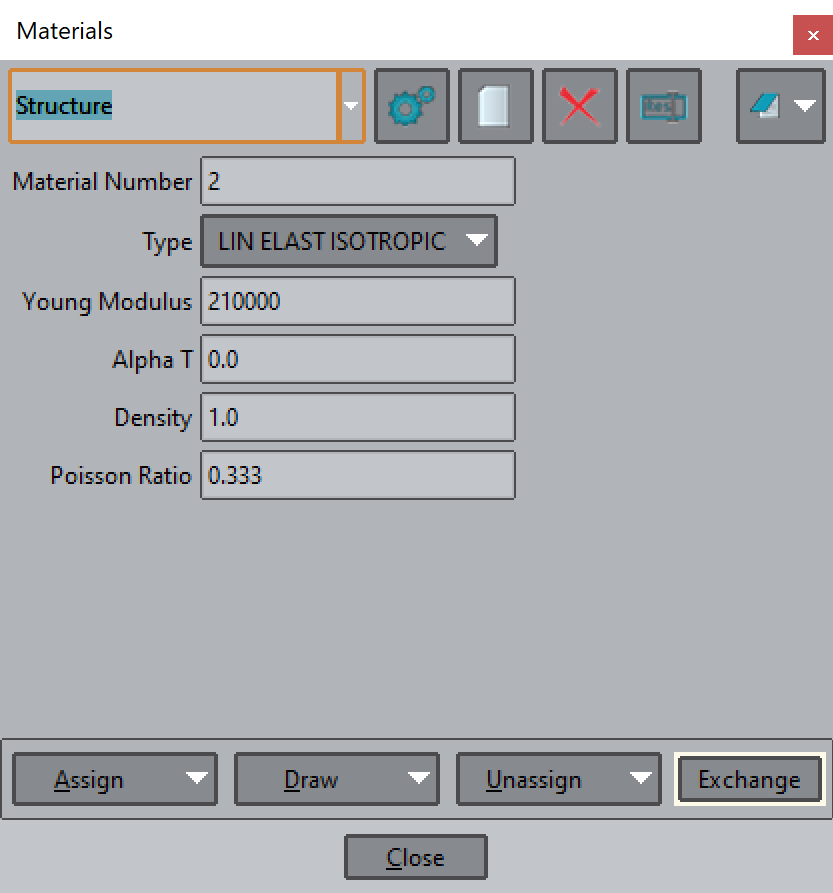
\includegraphics[width=60mm]{images/GiD_materials.png}
  \caption{material properties menu}
  \label{fig:GiDMaterialsMenu}
\end{figure}

%%%%%%%%%%%%%%%%%%%%%%%%%%%% GiD - optimization %%%%%%%%%%%%%%%%%%%%%%%%%
\subsubsection{Optimization}
If the user wants to execute the optimization algorithm, it can be found under \texttt{Data} $\rightarrow$ \texttt{Problem Data} $\rightarrow$ \texttt{Sensitivity Analysis}. Then select the \texttt{Structural Optimization} tab at the top of the menu. See Figure \ref{fig:GiDOptimizationMenu}. The user can specify the sensitivity analysis type, objective function, displacement direction, differencing method, perturbation, number of iterations, and factor of change. The recommended number of iterations is 10, and the recommended factor of change is 5. All other parameters have been discussed previously.

\begin{figure}[ht]
  \centering
  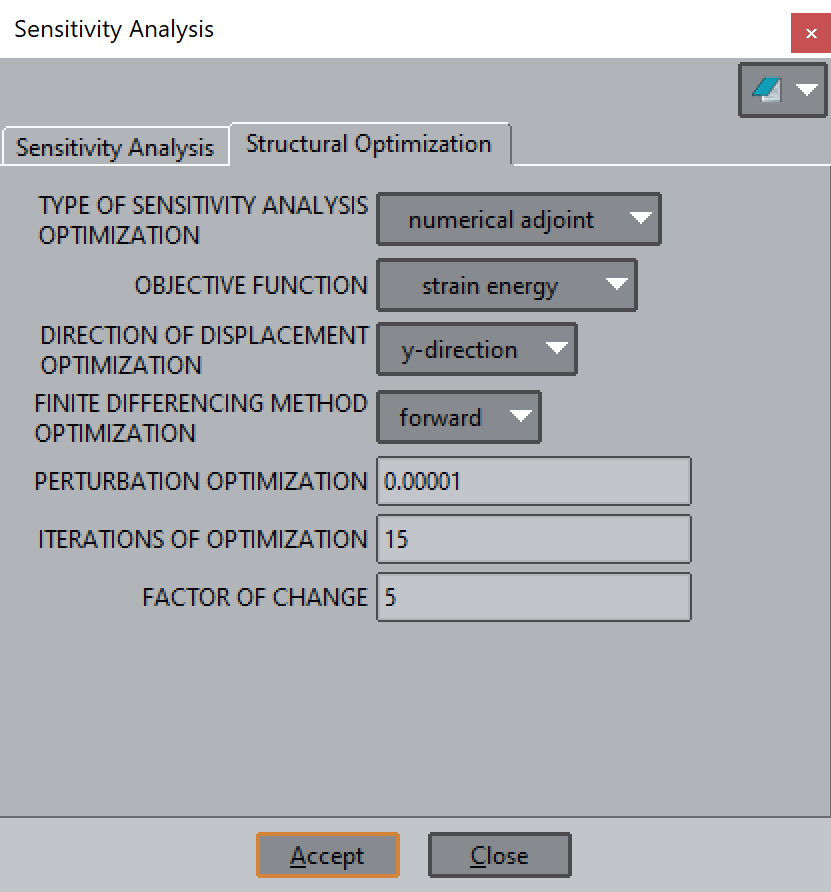
\includegraphics[width=60mm]{images/GiD_optimization.png}
  \caption{optimization menu}
  \label{fig:GiDOptimizationMenu}
\end{figure}

The optimization algorithm could be improved, as mentioned in Section \ref{section:optimization}. It is currently unstable if too many iterations are utilized; therefore, it is best to keep the iteration number at or below 10. The ideal factor of change will likely vary depending on the absolute size of the geometry created in GiD.

%%%%%%%%%%%%%%%%%%%%%%%%%%%% GiD - output %%%%%%%%%%%%%%%%%%%%%%%%%
\subsubsection{Output}
Now that all of the necessary information has been entered into GiD, ensure that the current file has been saved. Then, click \texttt{Calculate} $\rightarrow$ \texttt{Calculate}. This will generate a folder ending in \texttt{.gid}. There will be a \texttt{.dat} file within this folder. This file is what is read in from Matlab in the \texttt{main.m} driver file.  

\end{document}